%-----------------------------------------------------------------------------%
\chapter{IMPLEMENTASI DAN PENGUJIAN}
%-----------------------------------------------------------------------------%

\vspace{4.5pt}

\section{Lingkungan Implementasi}
Pada bagian ini dijelaskan mengenai spesifikasi perangkat keras dan kondisi lingkungan perangkat lunak yang digunakan selama proses implementasi dekomposisi dan pengujian.\\

\subsection{Spesifikasi Perangkat Keras}
Berikut spesifikasi perangkat keras untuk proses implementasi dekomposisi:

\begin{enumerate}[leftmargin=1.3cm]
	\item Nama Produk : Macbook Air 2020 
	\item Processor : Apple M1 8 Core CPU
	\item Memori : 8 GB
	\item Penyimpanan : 256 GB \\
\end{enumerate}


\subsection{Lingkungan Perangkat Lunak}
Berikut lingkungan perangkat lunak:

\begin{enumerate}[leftmargin=1.3cm]
	\item Sistem Operasi: macOS Ventura
	\item IDE : Visual Studio Code, GoLand 
	\item Tools : Dbeaver, Postman, Docker, Primate
	\item Bahasa Pemrograman: Python 3.8.2rc2, Go v1.20.4 \\
\end{enumerate}

\section{Implementasi Proses Clustering}
Pada bagian ini, dijelaskan mengenai proses, fungsi, dan metode yang digunakan dalam proses clustering untuk menemukan kelompok service di aplikasi monolitik yaitu Odoo.

\subsection{Pengambilan Source Code}
Proses ini pengambilan source code aplikasi Odoo bisa melalui source code repository di github.com. Source code tersebut digunakan untuk proses clustering dan proses dekomposisi dari monolitik ke microservice. Pada tugas akhir ini menggunakan Odoo v16 pada commit yang bisa direferensikan SHA1 375d0db3. 
\begin{lstlisting}[style=mystyle, language=sh, caption={Shell Script Git untuk pengambilan source code}]
$ git init
$ git remote add origin https://github.com/odoo/odoo
$ git fetch origin 375d0db3694419942a95e58212295b4186085e61:refs/remotes/origin/16.0 --depth=1
$ git checkout 375d0db3694419942a95e58212295b4186085e61
\end{lstlisting} 

\subsection{Pembuatan Call Graph}
Untuk membuat call graph dari source code aplikasi dapat menggunakan alat PyCG. PyCG harus terlebih dahulu di install bisa melalui pip. PyCG menganalisis kode program Python melalui package yang diberikan, untuk nama folder / package yang mengandung karakter "." harus diubah menjadi karakter lain karena PyCG membacanya dalam bentuk package Python. 

Proses analisis  dilakukan pada package odoo.addons dengan pengecualian folder test(pengujian). Hasil PyCG berupa .json yang kemudian diproses selanjutnya, proses ini membutuhkan waktu yang cukup lama karena besarnya aplikasi.
\begin{lstlisting}[style=mystyle, language=sh, caption={Shell Script untuk pembuatan call graph}]
$ pip install pycg
$ py_files=$(find addons -type f -name "*.py"  -not -path "*/tests/*")
$ pycg  --package addons  $py_files -o odooAddons.json
\end{lstlisting}

\begin{center}
	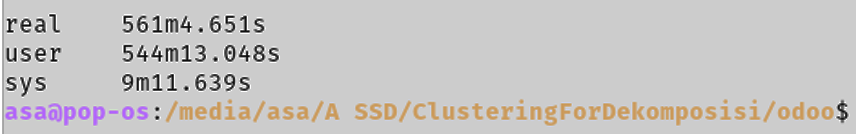
\includegraphics[width=10cm]{img/bab_4/hasil_run_pycg.png}
	\captionof{figure}{Waktu pembuatan call graph dengan PyCG}
	\label{fig:hasil_run_pycg}
\end{center}

Berikut adalah hasil dari scan yang dibuat PyCG. Dapat dilihat ada panggilan fungsi randint dari package random. Dari data ini tidak dapat diketahui apakah hubungan itu berupa module, class atau metode, untuk itu diproses selanjutnya akan menghilangkan informasi yang tidak penting dalam pengelompokan.

\begin{center}
	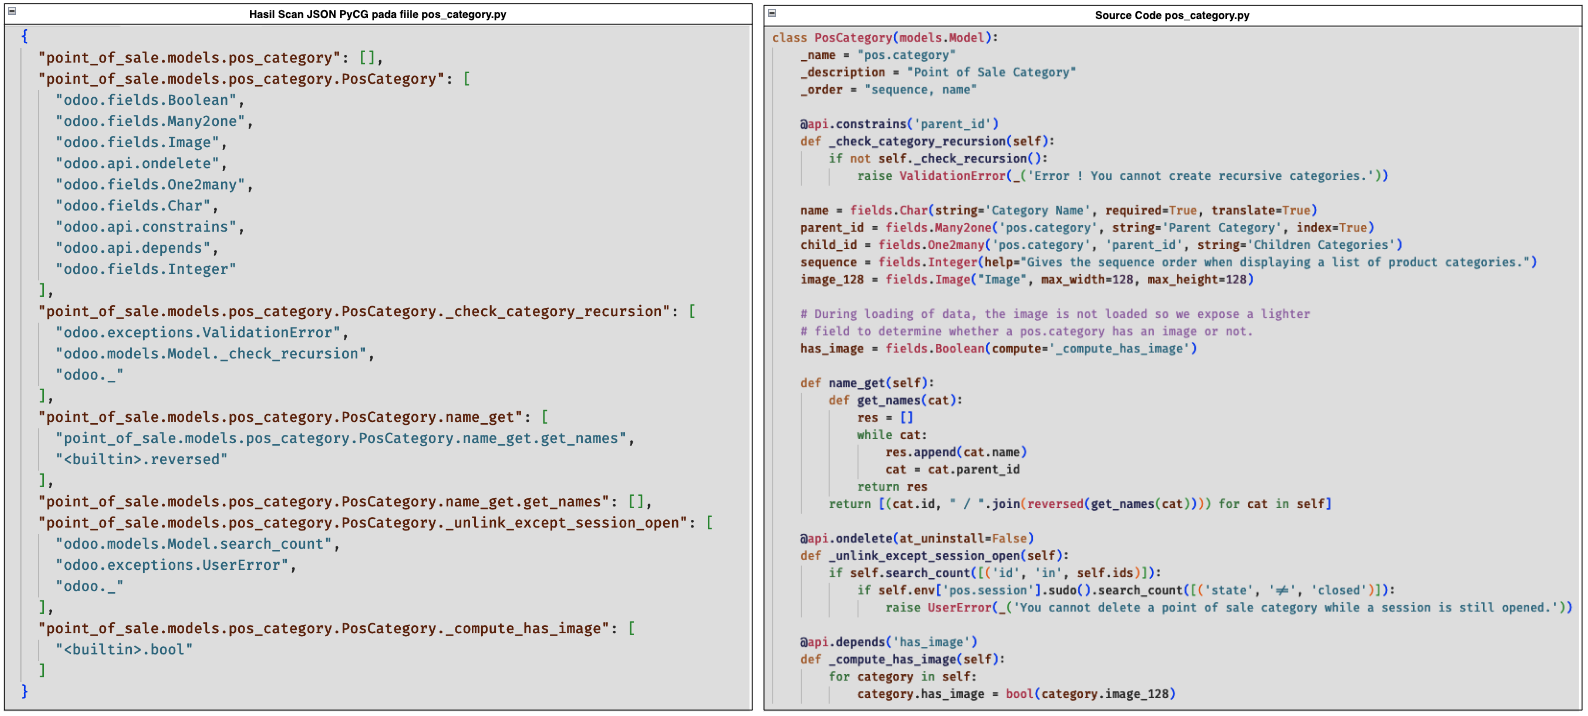
\includegraphics[width=14cm]{img/bab_4/hasil_scan_pycg.png}
	\captionof{figure}{Perbandingan hasil PyCG dengan Kode Program Aslinya}
	\label{fig:hasil_scan_pycg}
\end{center}

\subsection{Ekstraksi Dependency Model}
Pada proses ini dimulai dari menentukan path dimana kode program disimpan, kemudian karena terdapat 2 lokasi addons maka dibuat symbolic link dari addons ke odoo/addons agar inspect bisa mencari addons. Pencarian dimulai mencari module Python yang ada di file *.py, hasilnya module dibuka dengan inspect dan dicari class 'odoo.models.MetaModel'. Dari class tersebut akan memiliki atribut {\_}name, {\_}inherit/{\_}inherits, attribute{\_}rel, dan comodel{\_}name. Atribut ini dapat diekstraksi untuk membuat graph keterhubungan / ketergantungan antara module.

\begingroup
\setlength{\LTleft}{-20cm plus -1fill}
\setlength{\LTright}{\LTleft} % 13 cm
\begin{small}
	\begin{longtable}{|p{4cm}|p{3cm}|p{6cm}|}
		\caption{Daftar Metode untuk melakukan ekstraksi \textit{Dependency Module} }\\
		\hline
		\textbf{Metode / Fungsi} & \textbf{Parameter} & \textbf{Keterangan}\\
		\endfirsthead
		
		\hline  

		walkTroughFolder
		& folderSC,filterExt
		 & Fungsi rekursif untuk mencari daftar file di dalam folder hingga sub-folder dengan extensi yang tertentu  \\

		 \hline  
		
		 pathToModule
		& file, removeFile=True
		 &  Mengubah path slash menjadi dot python dan menghapus nama file jika diperlukan \\
		
		 \hline

		scanModuleWithInspect
		& modulePath
		 &  Membuat daftar class dari nama module dan hasilnya berisi nama model, inherit model, dan relasi attribute,  \\
		\hline  

		searchDependency
		& module
		 & Membuat graph dari daftar class yang dihasilkan scanModuleWithInspect \\
		\hline  

	\end{longtable}
\end{small}
\endgroup

\begin{center}
	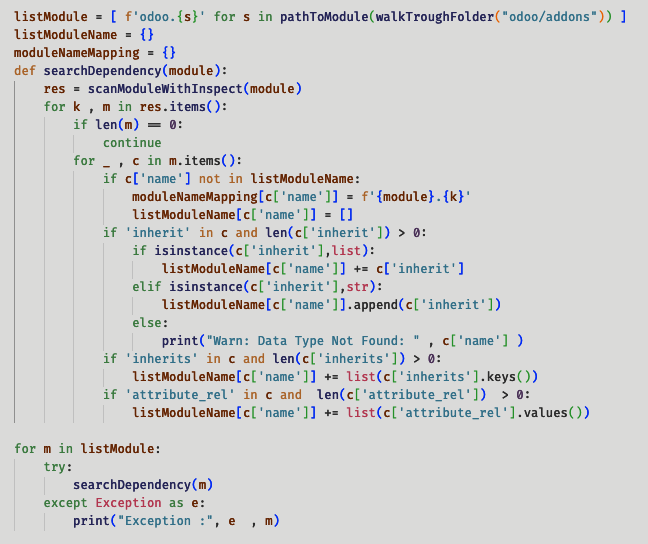
\includegraphics[width=14cm]{img/bab_4/def_inspect_1.png}
	\captionof{figure}{Implementasi Ekstraksi Model dengan inspect}
	\label{fig:def_inspect_1}
\end{center}

Pada gambar \ref{fig:def_inspect_1}, proses yang dilakukan yaitu membuat daftar nama module python yang dari path "odoo/addons" dengan bentuk nama module "odoo.nama{\_}model". Terdapat 2 variabel yaitu listModuleName untuk menyimpan relasi sebuah model dengan model lainnya dan variabel moduleNameMapping untuk memetakan nama dari nama model menjadi nama module yang dikenal oleh Python seperti nama model 'sale.order' dapat dipetakan menjadi 'odoo.addons.sale.models.sale{\_}order'.

Proses pencarian dilakukan satu  per satu dari daftar module yang ada di variabel listModule. Fungsi searchDependency berfungsi untuk mengubah daftar class dan atributnya yang dihasilkan oleh scanModuleWithInspect untuk bisa dibuat menjadi keterhubungan karena dalam module bisa memiliki banyak model / class dan bisa dipetakan dari nama model menjadi nama module Python.  

\begin{center}
	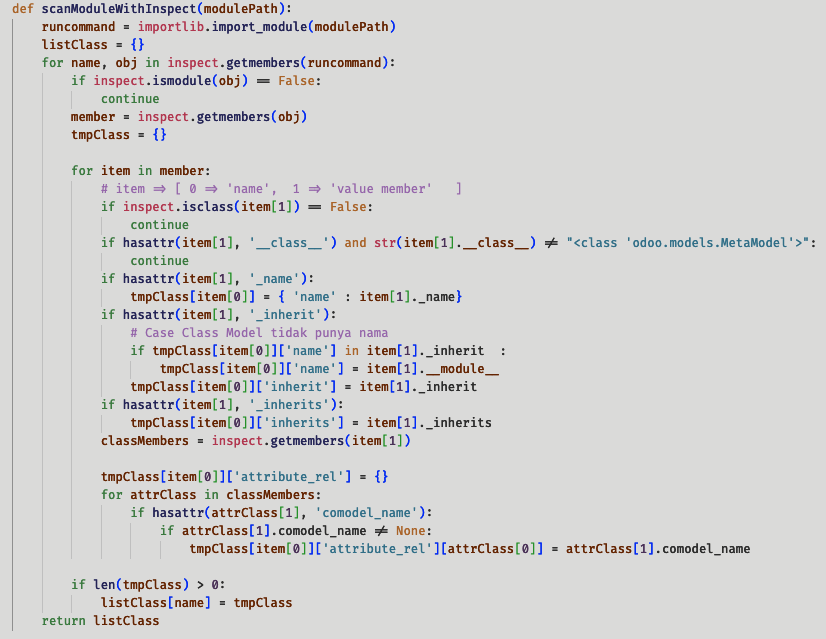
\includegraphics[width=14cm]{img/bab_4/def_inspect_2.png}
	\captionof{figure}{Implementasi Ekstraksi Model dengan inspect Lanjutan}
	\label{fig:def_inspect_2}
\end{center}

Fungsi scanModuleWithInspect yang dapat dilihat pada gambar \ref{fig:def_inspect_2} memiliki masukan berupa string untuk alamat module dengan bentuk dot path seperti "odoo.addons.product".  Untuk mengetahui isi dari sebuah kode program python harus dilakukan proses pembacaan kode program, pembacaan ini dimulai dari memasukan alamat direktori tempat dimana kode program berada, melalui import{\_}module. Import module membantu untuk mengambil sebuah module secara dinamik, hasilnya berupa objek Python yang berisi module dari alamat yang dimasukan. Pada bahasa pemrograman Python hampir semua hal adalah sebuah objek, sehingga dari objek bisa ditentukan tipe data apa yang dimiliki objek tersebut.

Module bisa memiliki banyak module \verb|->| sub-modul(file) \verb|->| class / def / var /object. Untuk mengetahui apakah sebuah module memilikinya maka digunakan \verb|inspect.getmember|. Hasil keluaran \verb|inspect.getmember| berupa array dimana \verb|['nama_objek', isi_object]|. 

Setiap member bisa berisi bermacam-macam data dan berupa metadata. Apabila module memiliki sub-module make dicari kembali class-nya dari sub-module tersebut. Fungsi ini hanya berfokus mencari class pada sebuah module/sub dengan tipe odoo.models.MetaModel, jika terdapat class yang memiliki tipe MetaModel. Maka dilakukan pengecekan apakah object tersebut memiliki attribute {\_}name, {\_}inherit, {\_}inherits, attribute{\_}rel, dan comodel{\_}name. 

Masing-masing atribute ini seperti yang sudah dijelaskan pada tinjauan objek memiliki makna yang penting untuk menentukan relasi antar class. Attribute kemudian simpan di variabel dictionary(key,value) dengan key adalah nama module dan relasi serta namanya, isi datanya berupa string yang merepresentasikan sebuah nama model di Odoo seperti 'res.users'. 

\begin{center}
	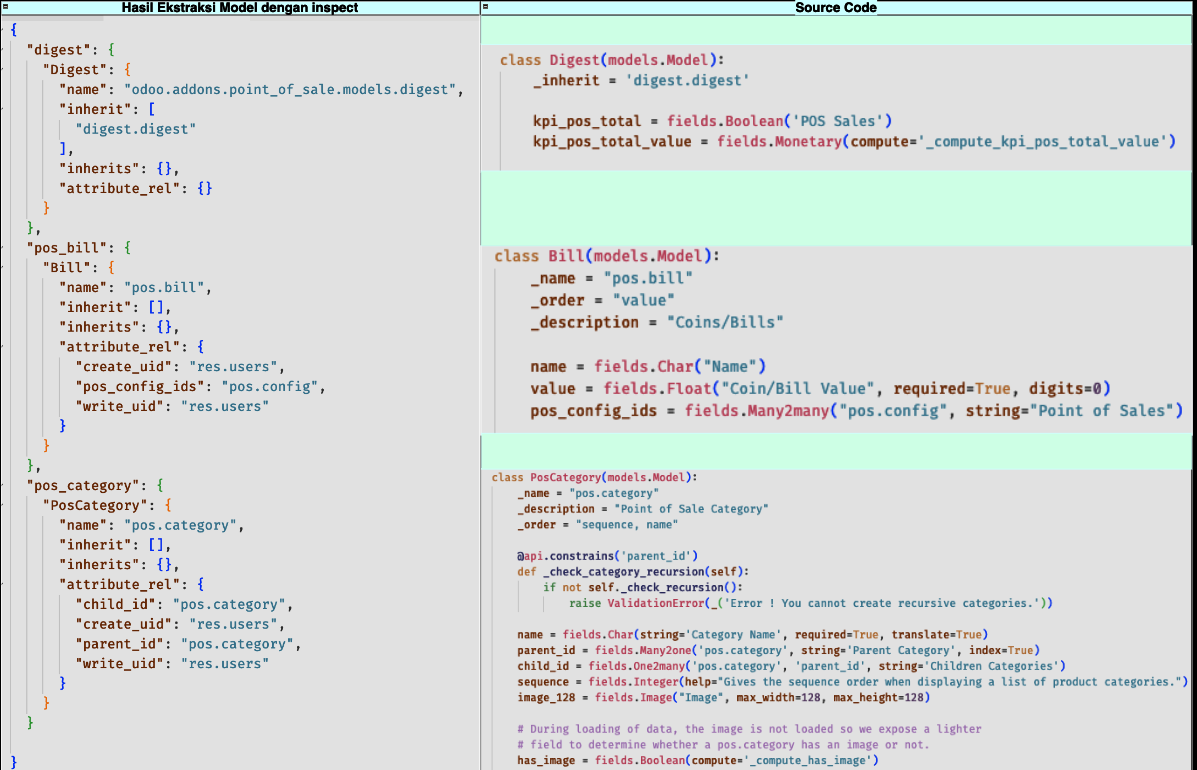
\includegraphics[width=14cm]{img/bab_4/def_inspect_3.png}
	\captionof{figure}{Contoh Informasi yang diekstraksi dari Model}
	\label{fig:def_inspect_3}
\end{center}

Informasi seperti di gambar \ref{fig:def_inspect_3} harus diubah oleh fungsi searchDependency dan hasilnya disimpan pada variabel listModuleName dan moduleNameMapping.
Hasil dari pembuatan dependency model ini yaitu berupa graph yang disimpan di listModuleName contohnya seperti pada gambar \ref{fig:def_inspect_4}. Graph ini baru dikelompokan berdasarkan nama model yang diketahui Odoo. Name Model ini akan dipetakan menjadi nama module. Sehingga bisa dilakukan penggabungan antara hasil PyCG dan inspect.

\begin{center}
	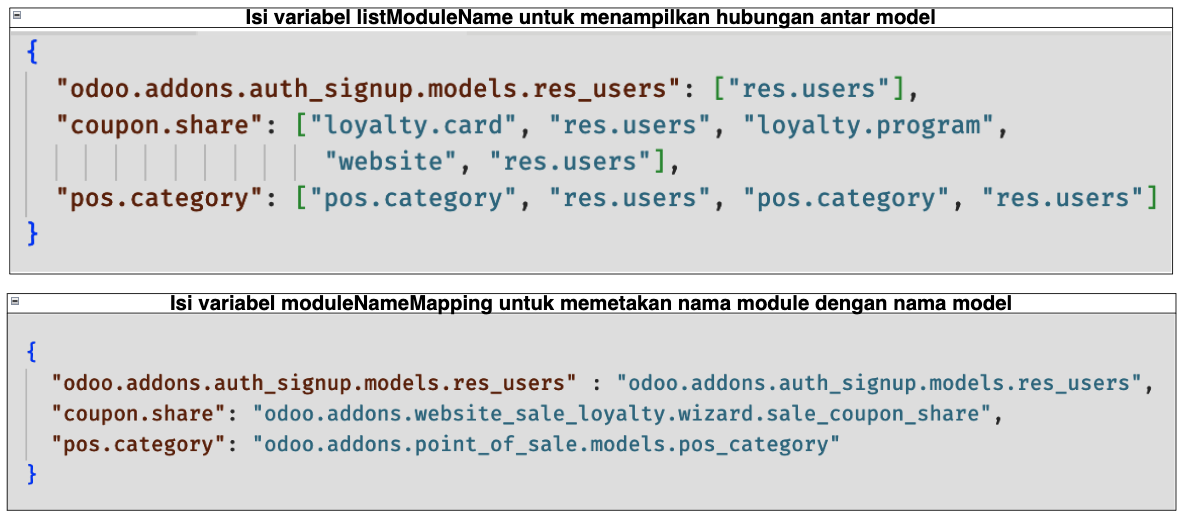
\includegraphics[width=14cm]{img/bab_4/def_inspect_4.png}
	\captionof{figure}{Hasil ekstraksi dari Model menggunakan inspect}
	\label{fig:def_inspect_4}
\end{center}

\subsection{Pengabungan Hasil Ekstraksi}
Hubungan ketergantungan yang sudah dihasilkan dari PyCG dan inspect, diproses dan dijadikan satu kesatuan sebelum dilakukan proses clustering. Hal yang diproses seperti menghapus node yang tidak terpakai atau diluar dari Odoo seperti keterhubungan dengan library ke-3.  

\begingroup
\setlength{\LTleft}{-20cm plus -1fill}
\setlength{\LTright}{\LTleft}
\begin{small}
	\begin{longtable}{|p{4cm}|p{3cm}|p{6cm}|}
		\caption{Daftar Metode untuk pengabungan hasil ekstraksi}\\
		\hline
		\textbf{Metode / Fungsi} & \textbf{Parameter} & \textbf{Keterangan}\\
		\endfirsthead
		
		\hline  

		loadJSON
		& path
		 & Membuka file json dari suatu path  \\

		 \hline  

		 getListRootPackage
		& path
		 & Membuat daftar module/package dari folder path bila folder tersebut memiliki Python. \\

		 \hline  

		 addPrefixFolder
		& cg,root,listPackage
		 & Menambahkan awal root dari call graph yang dihasilkan dari PyCG(JSON) dan disatukan berdasarkan nama modulenya  \\
		 
		 \hline  

		 mergeCGOdooWithAddons
		& cgOdoo,cgAddons
		 & Mengabungkan call graph dari odoo dan addons yang sudah memiliki prefix  \\


		 \hline  

		 filterCGNode
		& cgSource
		 & Menghapus node atau hubungan yang tidak di dalam module addons atau base pada graph \\

		 \hline
		
		 updateCGwInspect
		& listModuleName, moduleNameMapping, callGraph
		 & Mengabungkan hasil relasi yang ditemukan di library inspect ke call graph  \\

		 \hline
	\end{longtable}
\end{small}
\endgroup

\begin{center}
	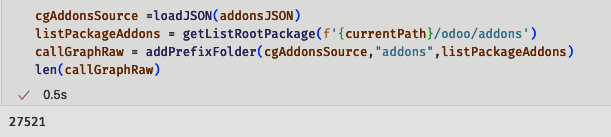
\includegraphics[width=10cm]{img/bab_4/ekstraksi_1.png}
	\captionof{figure}{Proses pembacaan file JSON dan penambahaan prefix}
	\label{fig:ekstraksi_1}
\end{center}

Proses penggabungan dimulai dengan mengimport file JSON yang dihasilkan oleh PyCG. File JSON tersebut diubah menjadi bentuk call graph di dictionary(key,value). Nama node yang dihasilkan PyCG tidak lengkap karena dilakukan scan melalui odoo/addons maka tidak ada prefix atau parentnya yang lengkap, untuk itu dilakukan penambahaan nama module didepan nama node "addons" sehingga yang awalannya langsung merupakan nama package / addons seperti "product.models" maka menjadi "addons.product.models". Tujuan dilakukan ini agar node di graph dari PyCG memiliki tingkatan yang sama dengan nama package odoo. Penambahan ini menggunakan fungsi addPrefixFolder dan getListRootPackage.

\begin{center}
	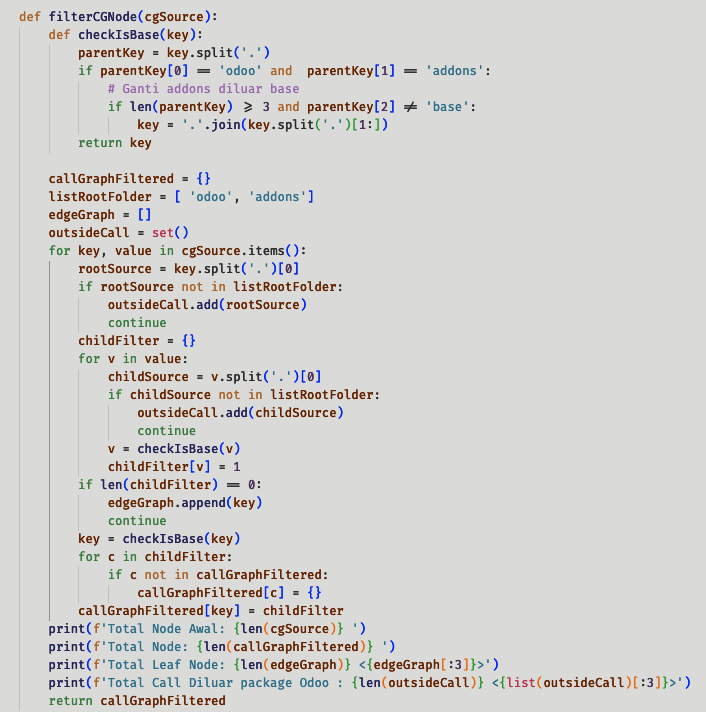
\includegraphics[width=13cm]{img/bab_4/ekstraksi_2.png}
	\captionof{figure}{Isi fungsi filterCGNode}
	\label{fig:ekstraksi_2}
\end{center}

Isi dari graph dilakukan pembuangan pada node yang tidak diinginkan untuk dikelompokan, karena tugas besar ini berfokus pada mengelompokan pada bagian module addons / proses bisnis maka setiap relasi ke package diluar  odoo dan addons akan dihilangkan dari graph. Proses ini dilakukan oleh fungsi filterCGNode, fungsi tersebut membuat graph baru dari graph yang memiliki informasi call graph original dan menghapus node yang tidak memiliki hubungan apapun. Fungsi filterCGNode juga memberikan nilai setiap hubungan call sebesar 1, nilai ini akan digunakan sebagai weight atau jumlah call ke suatu node. Call Graph yang dihasilkan dari PyCG tidak memberikan jumlah call sehingga semua call diasumsikan memiliki nilai panggilan sebesar 1. Proses pengubahan dan penyerderhanaan graph dilakukan oleh fungsi filterCGNode.

\begin{center}
	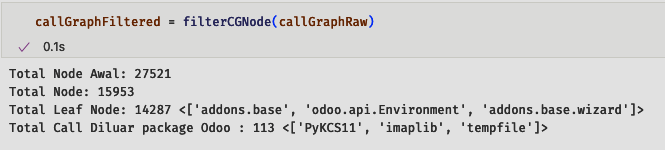
\includegraphics[width=9cm]{img/bab_4/ekstraksi_3.png}
	\captionof{figure}{Hasil akhir node dari yang sudah digabungkan dan dibersihkan}
	\label{fig:ekstraksi_3}
\end{center}

Pada gamber \ref{fig:ekstraksi_3} dapat terlihat jumlah awal node yang awalnya sebesar 27.521 setelah difilter menjadi sebesar 15.953. Node leaf yaitu fungsi yang ditemukan tidak memanggil node lain, untuk itu node tersebut dihilangkan. Proses selanjutnya yaitu mengabungkan call graph dengan hasil inspect, sebelumnya hasil inspect disimpan pada variabel listModuleName dan moduleNameMapping. 

\begin{center}
	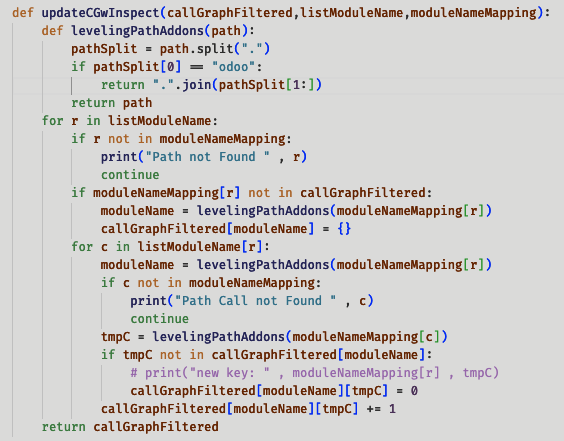
\includegraphics[width=10cm]{img/bab_4/ekstraksi_4.png}
	\captionof{figure}{Isi fungsi updateCGwInspect}
	\label{fig:ekstraksi_4}
\end{center}

Pada inspect dapat diketahui jumlah berapa hubungan antara sebuah module, seperti misalkan ada model yang memiliki 2 attribute yang disebut 'write{\_}uid' untuk menandakan siapa  yang mengupdate data dengan relasi res.users dan 'create{\_}uid' untuk menandakan siapa  yang membuat data dengan relasi res.users. Selain itu nama model dari inspect akan disesuaikan dengan moduleNameMapping agar pencarian model 'pos.category' dapat menjadi 'odoo.addons.point{\_}of{\_}sale.models.pos{\_}category'. Proses penggabungan dengan inspect dilakukan oleh fungsi updateCGwInspect.

\begin{center}
	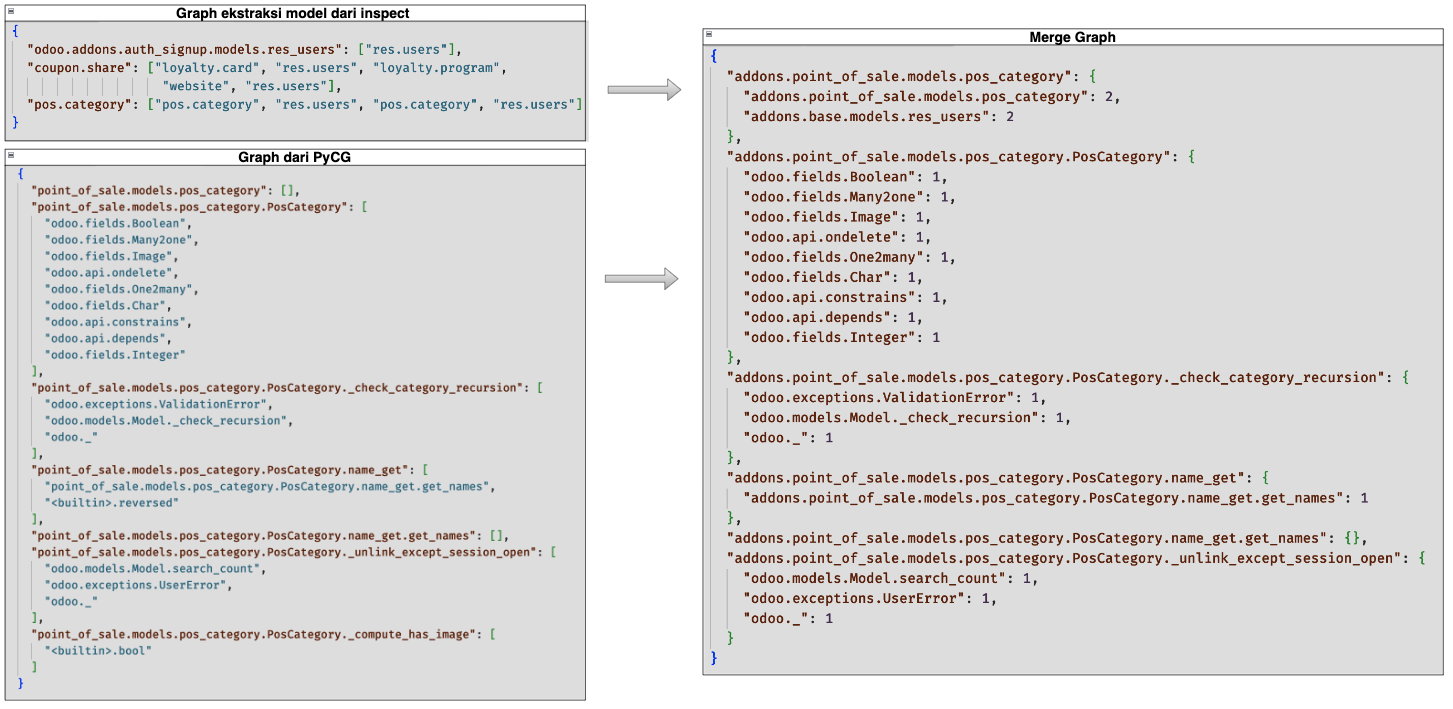
\includegraphics[width=14cm]{img/bab_4/ekstraksi_5.png}
	\captionof{figure}{Ilustrasi Hasil Gabungan Graph}
	\label{fig:ekstraksi_5}
\end{center}

\subsection{Optimisasi Hasil Ekstraksi}
Hasil graph yang sudah digabungkan dari hasil ekstraksi harus diproses kembali agar pengelompokan yang dilakukan oleh Hierarchical Clustering terarah. Pada Tugas akhir ini pengelompokan dilakukan berdasarkan proses bisnisnya, proses bisnis tersebut berada pada module yang dinamakan 'addons'. Setiap panggilan kepada suatu addons / node harus diagregasikan untuk dijadikan \textit{weight} yang berkisar 0 (tidak ada relasi) hingga 1 (memiliki relasi yang kuat)


\begingroup
\setlength{\LTleft}{-20cm plus -1fill}
\setlength{\LTright}{\LTleft}
\begin{small}
	\begin{longtable}{|p{4cm}|p{3cm}|p{6cm}|}
		\caption{Daftar Metode untuk optimisasi hasil ekstraksi}\\
		\hline
		\textbf{Metode / Fungsi} & \textbf{Parameter} & \textbf{Keterangan}\\
		\endfirsthead
		
		 \hline
		 initKeyCG
			& -
		 & Membuat daftar key untuk graph addons kecuali module test dan l10n  \\
		 
		 \hline
		 checkNameKey		 
			& k
		 & Mengecek apakah name pada sebuah nama module memiliki module yang tidak perlu dikelompokan seperti 'tests', 'testing','test', 'l10n' \\

		 \hline
		 updateCGWeight
		& callGraphFiltered, callGraphWeight
		 & Membuat call graph yang memiliki nilai berbobot (weighted graph) berdasarkan jumlah panggilan(call) dengan cara menjumlahkan call yang dipanggil dari module \\

		 
		 \hline 
		 cleanUpCG
			& callGraph
		 & Menghilangkan call yang rendundan dan  menyimpan informasi panggilan internal di variabel yang terpisah\\

		 \hline
		 removeNotConnectedNode
		& callGraph
		 & Menghapus node parent yang tidak terhubung ke node lain  dan memastikan node graph yang dibentuk lengkap\\
		

		 \hline  
		createAdjacentMatrix
		& graphSource
		 & Membuat adjacency matrix dari graph  \\
		
		 \hline  
		 
	\end{longtable}
\end{small}
\endgroup

Untuk mengetahui jumlah panggilan keluar atau panggilan didalam module maka graph yang sudah disatukan sebelumnya diubah menjadi bentuk tree. Dengan bentuk tree ini bisa dilakukan perhitungan jumlah panggilan dan relasinya. Tree dibuat dengan class NodeCG,seperti pada gambar \ref{fig:optimasi_1}. Proses perubahan graph pada gambar \ref{fig:optimasi_2} dimulai dari membentuk root dengan nama "odoo" kemudian mengubah semua relasi setiap node relasi baru dengan fungsi setRelation pada class NodeCG. Apabila nama dari relasi memiliki module yang berkaitan dengan testing atau lokalisasi seperti 'addons.product.tests' maka relasi 'addons.product.tests' tidak ditambahakan pada odooTree. 

\begin{center}
	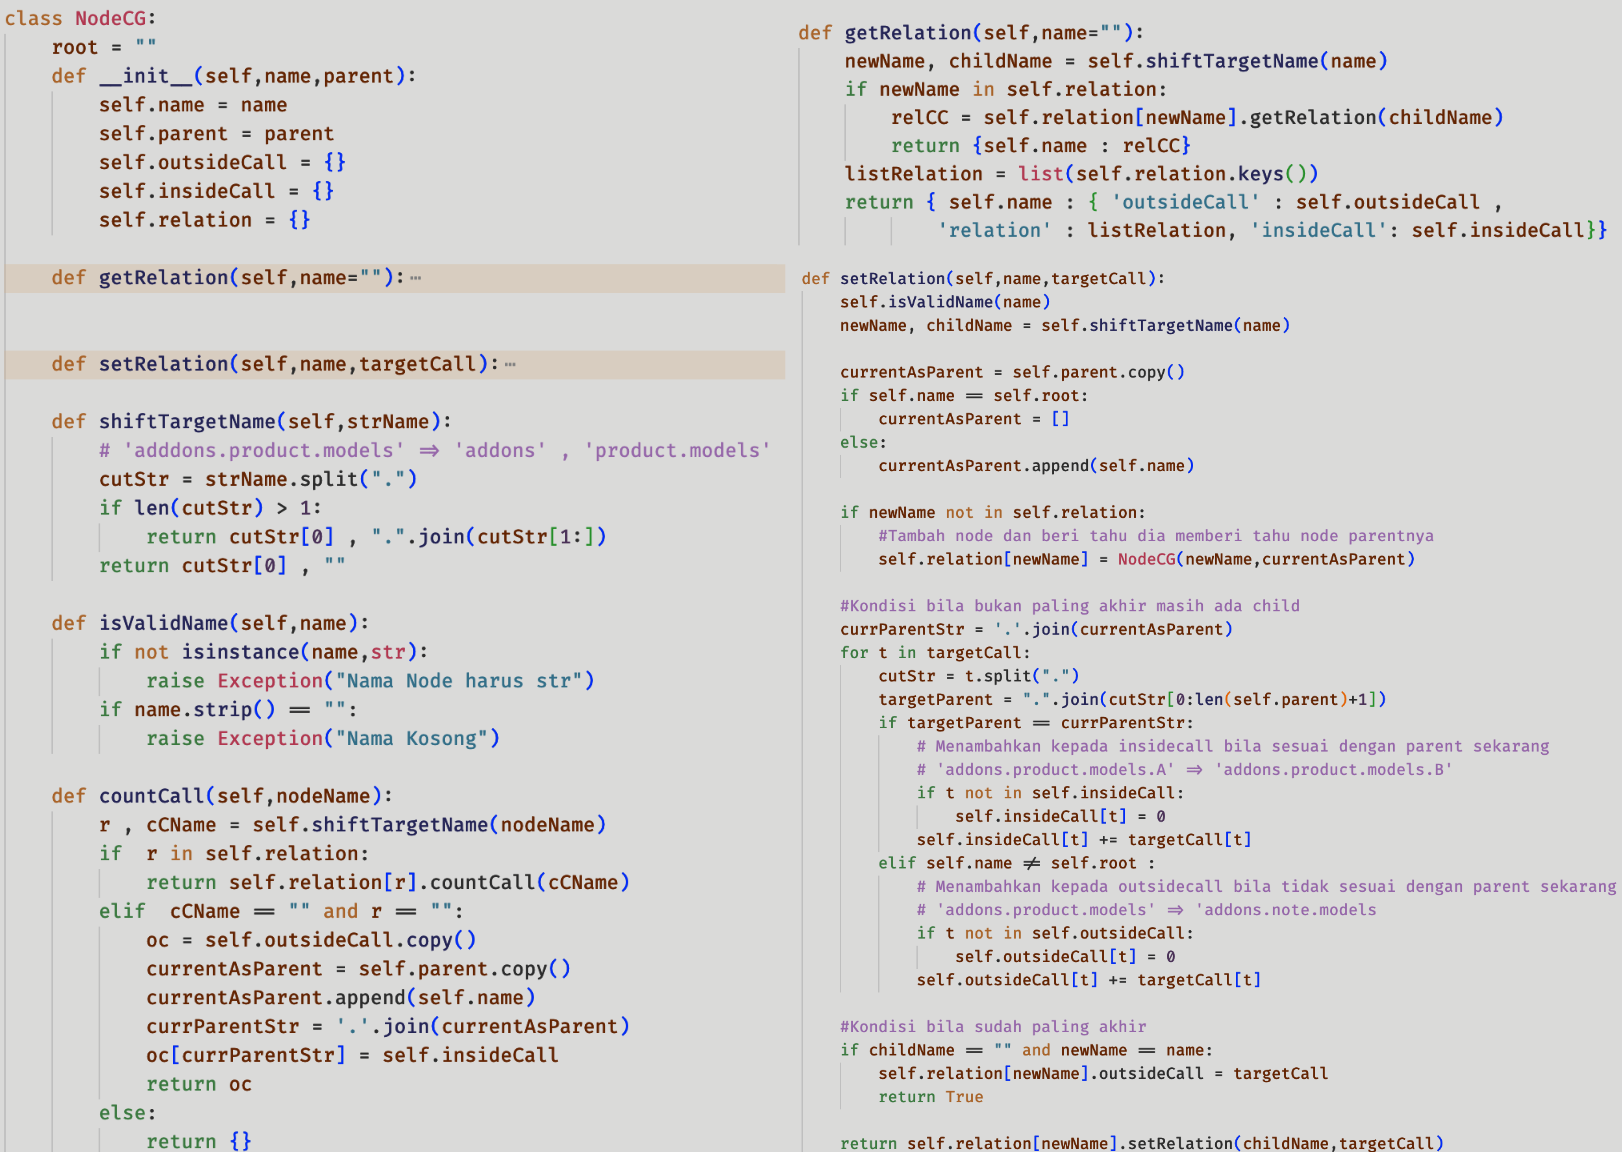
\includegraphics[width=14cm]{img/bab_4/optimisasi_1.png}
	\captionof{figure}{class NodeCG untuk menghitung weight}
	\label{fig:optimasi_1}
\end{center}

\begin{center}
	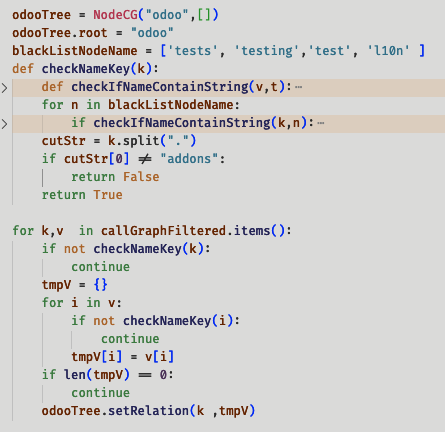
\includegraphics[width=9cm]{img/bab_4/optimisasi_2.png}
	\captionof{figure}{Proses perubahan graph di dictionary menjadi class NodeCG}
	\label{fig:optimasi_2}
\end{center}

Penambahan relasi node di tree yang dilakukan oleh fungsi setRelation yaitu berupa key string seperti 'addons.point{\_}of{\_}sale.model' dan isi relasi node. Fungsi setRelation membuat relasi baru didalam tree bila module tersebut belum ada, jika sudah ada relasi sebelumnya maka setRelation akan menggunakan relasi itu dan memperbarui isi relasi. Fungsi ini berhenti ketika sudah tidak ada child module seperti contohnya 'a.i' make child dari module 'a' adalah 'i' dan module 'i' tidak memiliki memiliki child. Hasil perubahan dari graph yang direpresentasikan dalam bentuk dictionary ke bentuk tree di NodeCG dapat dilihat pada gambar \ref{fig:optimasi_3}

\begin{center}
	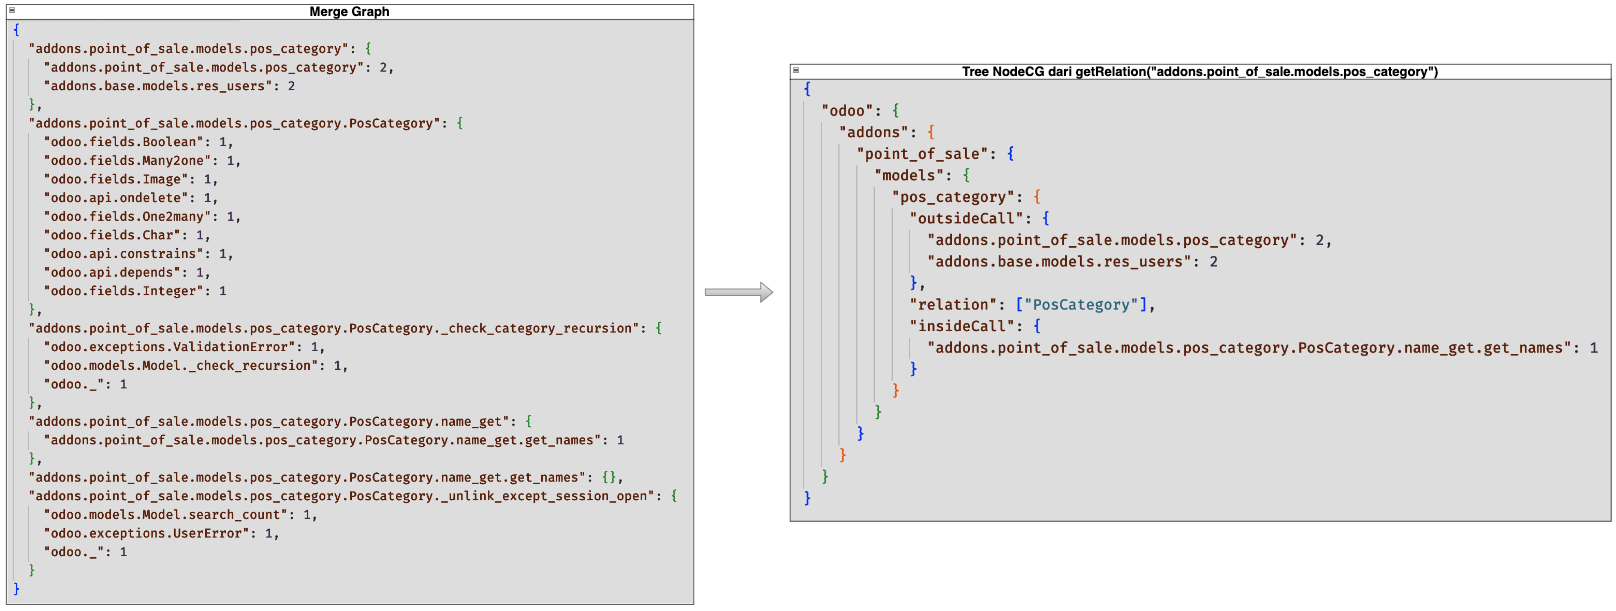
\includegraphics[width=12cm]{img/bab_4/optimisasi_3.png}
	\captionof{figure}{Ilustrasi Path dot menjadi bentuk Tree NodeCG}
	\label{fig:optimasi_3}
\end{center}

Proses selanjutnya yaitu membuat graph baru yang hanya berisi module addons, proses ini dilakukan oleh fungsi initKeyCG. Fungsi akan membaca direktori dari path odoo/addons dan hanya menambahkan bila module tersebut adalah package (folder). Kemudian graph baru diperbarui isi relasinya dengan fungsi updateCGWeight. Fungsi updateCGWeight menggunakan odooTree dan call graph baru. Kemudian dilakukan pengecekan apakah graph yang dibuat lengkap dan dibuat menjadi Adjacency Matrix.  Dari gambar \ref{fig:optimasi_4} dapat dilihat terdapat 335 objek yang akan dilakukan proses hierarchical clustering.

\begin{center}
	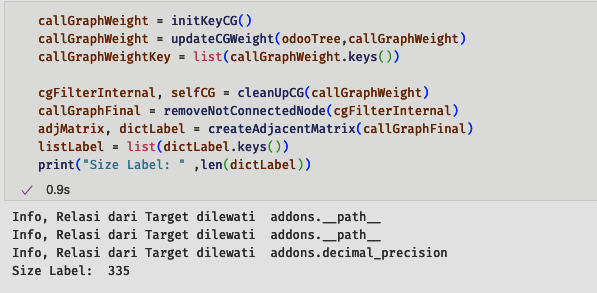
\includegraphics[width=9cm]{img/bab_4/optimisasi_4.png}
	\captionof{figure}{Proses Optimisasi Graph dan Pembuatan Adjacency Matrik}
	\label{fig:optimasi_4}
\end{center}

Hasil dari proses ini dapat dilihat pada gambar \ref{fig:optimasi_5}, dapat dilihat pengabungan panggilan yang diagregasikan berdasarkan module addons. Proses ini juga menghitung berapa relasi dalam dirinya sendiri, tujuan perhitungan ini untuk mengetahui berapa besar kohesi didalam module. Jumlah relasi kepada diri sendiri tidak ditambahkan pada Adjacency matrix, dan matriks yang dibuat juga dilakukan column-wise normalization seperti yang dijelaskan pada bagian Urutan Proses Global.  

\begin{center}
	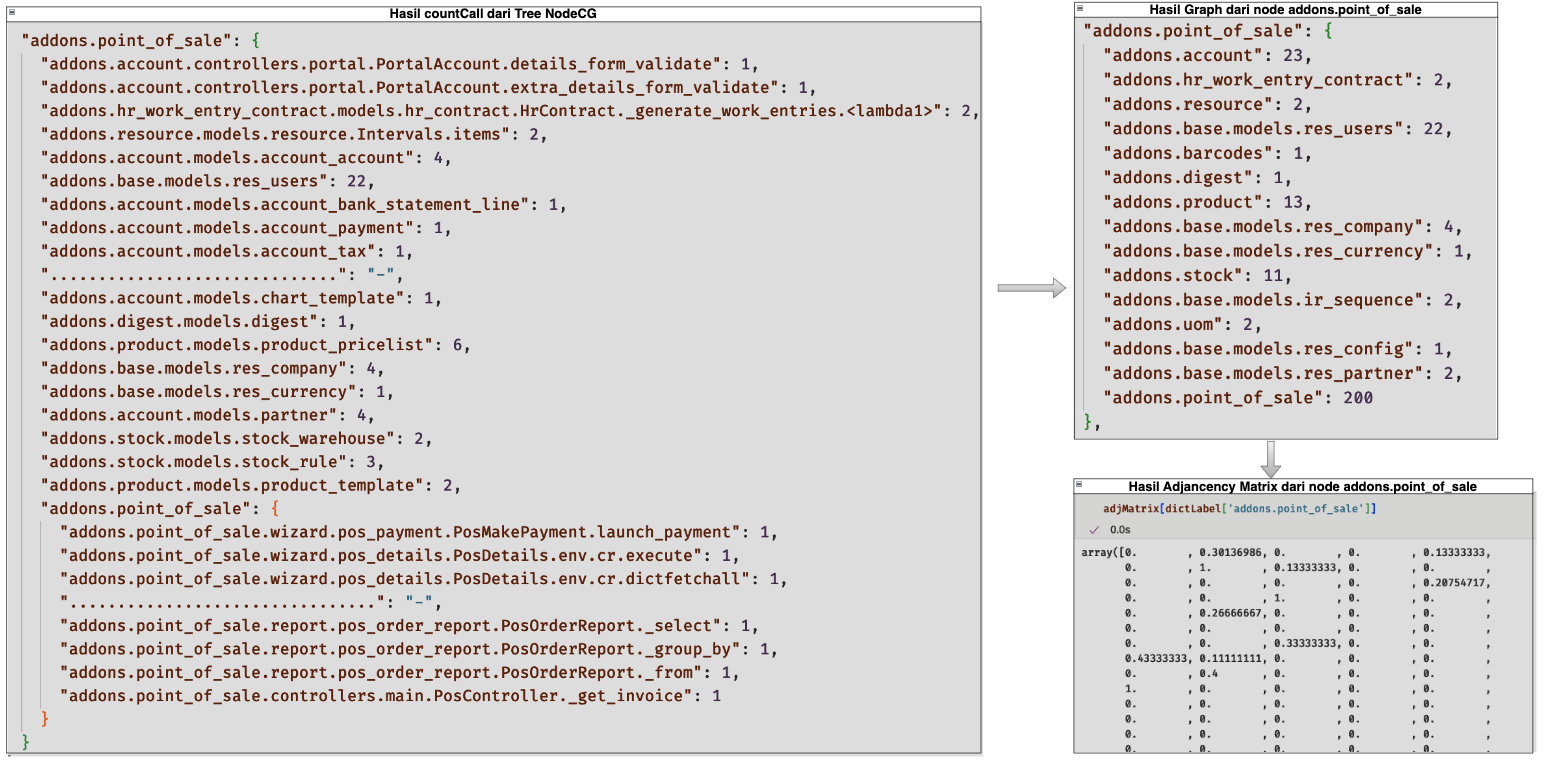
\includegraphics[width=14cm]{img/bab_4/optimisasi_5.png}
	\captionof{figure}{Ilustrasi Hasil Graph yang dapat dilakukan Proses Pengelompokan}
	\label{fig:optimasi_5}
\end{center}


\subsection{Hierarchical Clustering}
Proses ini dilakukan untuk menemukan pengelompokan dari adjacency matrix. Matrix adjacency(Matrix keterhubungan) harus dihitung untuk mendapatkan nilai kedekatannya, perhitungan tersebut menghasilkan Distance Matrix(Matrik kedekatan). Pada tugas akhir ini menggunakan nilai kedekatan berdasarkan nilai Jaccard dan Struktural Similarity. 

\begin{center}
	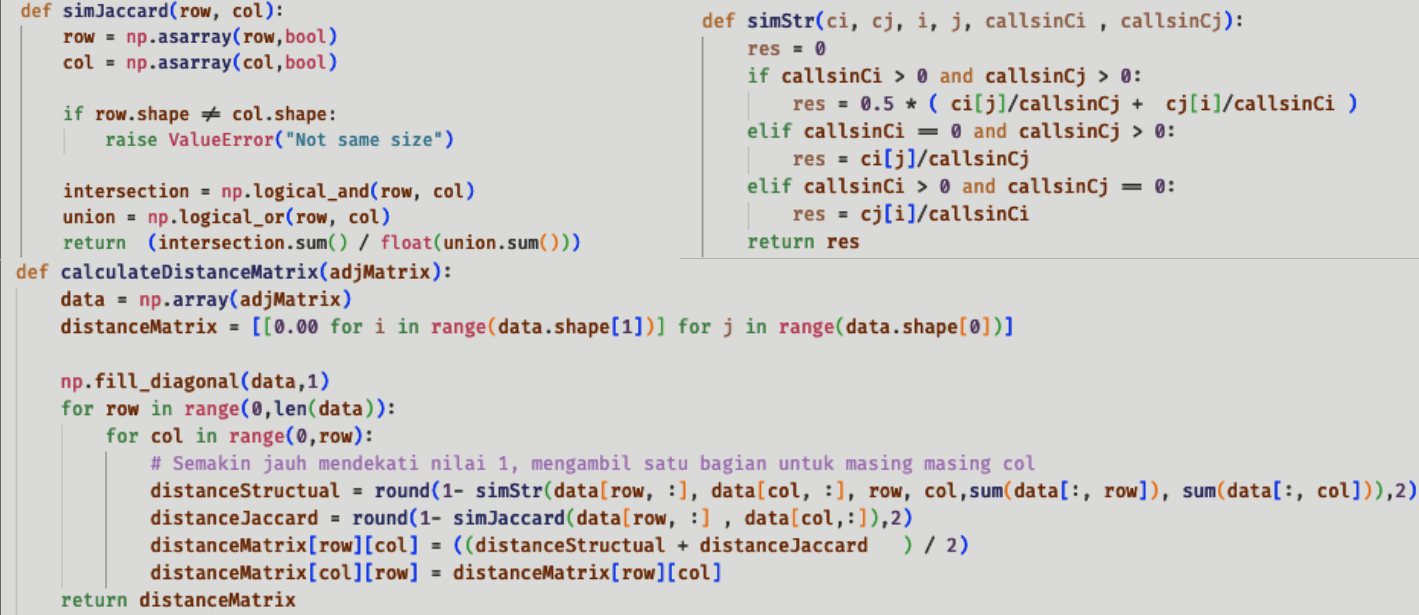
\includegraphics[width=12cm]{img/bab_4/hc_1.png}
	\captionof{figure}{Implementasi Perhitungan Distance Matrix dengan Jaccard dan Struktural Similarity}
	\label{fig:hc_1}
\end{center}

Matriks kedekatan bisa ditampilan dalam bentuk heatmap. Heatmap dapat memberikan bagaimana intensitas kedekatan antar module addons Odoo. Pada gambar \ref{fig:heatmap_gambar} dapat dilihat semakin kuning atau cerah maka semakin tinggi intensitas hubungannya sedangkan semakin hijau atau redup maka intensitas hubungannya rendah. heatmap ini dihasilkan dari matrix segitiga sehingga hasil dari heatmap sisi kiri sama dengan heatmap sisi kanan.

\begin{center}
	\includegraphics[width=7cm]{img/bab_4/HeatmapModule.png}
	\captionof{figure}{Heatmap yang menunjukan intensitas hubungan antar module/node}
	\label{fig:heatmap_gambar}
\end{center}


\begingroup
\setlength{\LTleft}{-20cm plus -1fill}
\setlength{\LTright}{\LTleft}
\begin{small}
	\begin{longtable}{|p{4cm}|p{3cm}|p{6cm}|}
		\caption{Daftar Metode untuk proses Clustering}\\
		\hline
		\textbf{Metode / Fungsi} & \textbf{Parameter} & \textbf{Keterangan}\\
		\endfirsthead
		
		\hline  

		simStr
		& ci, cj, i, j, callsinCi , callsinC
		 & Implementasi dari rumus 2.2  \\

		 \hline  

		 simJaccard
		& im1, im2
		 & Implementasi dari rumus 2.1   \\

		 \hline  

		 calculateDistanceMatrix
		& adjMatrix
		 & Menghitung distance matrix dengan masukan adjacency matrix  \\

		 \hline  

		 visualizeHeatmap
		& matrix, title
		 & Membuat visualisasi heatmap  \\

		 \hline  

		 calculateCluster
		& y, {\_}method
		 & Melakukan proses clustering dengan linkage function tertentu ({\_}method) dan distance matrix (y) \\

		 \hline
		
		 visualizeDendogram
		& z, {\_}method
		 & Menampilakan dendogram dari hierarchical clustering  \\

		 \hline
	\end{longtable}
\end{small}
\endgroup

Distance Matrix dimasukan kedalam fungsi calculateCluster dengan metode ada 3 yaitu average, min, max. Hasil cluster dari hierarchical clustering bisa divisualisasi dalam bentuk dendogram. Hasil dendogram memiliki distance/jarak antar module dan label module. Dari gambar \ref{fig:dd_single} module cenderung dikelompokan dengan jumlah yang kecil (1-2) dan ketika dihubungkan memiliki jarak yang jauh. Pada pendekatan \ref{fig:dd_complete} module dikelompokan dan memiliki ukuran module yang besar untuk setiap partisi/service. Sedangkan pendekatan \ref{fig:dd_avg} memiliki bentuk campuran antara ukuran module yang besar dan module yang berukuran kecil.

\begin{figure}[htbp]
	\centering
	\begin{minipage}{1\textwidth}
		\centering
		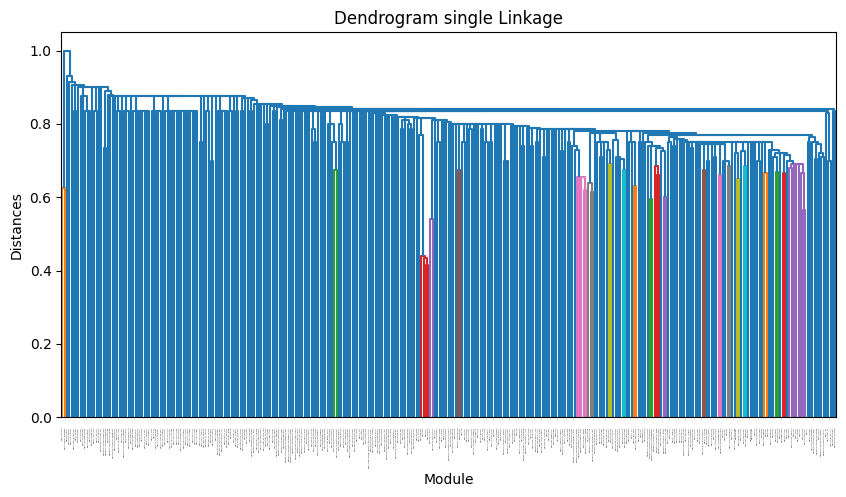
\includegraphics[width=1\textwidth]{img/bab_4/single_dd.png}
		\caption{Dendogram Single Linkage }
		\label{fig:dd_single}
	\end{minipage}\hfill	
\end{figure}

\begin{figure}[htbp]
	\centering
	\begin{minipage}{1\textwidth}
		\centering
		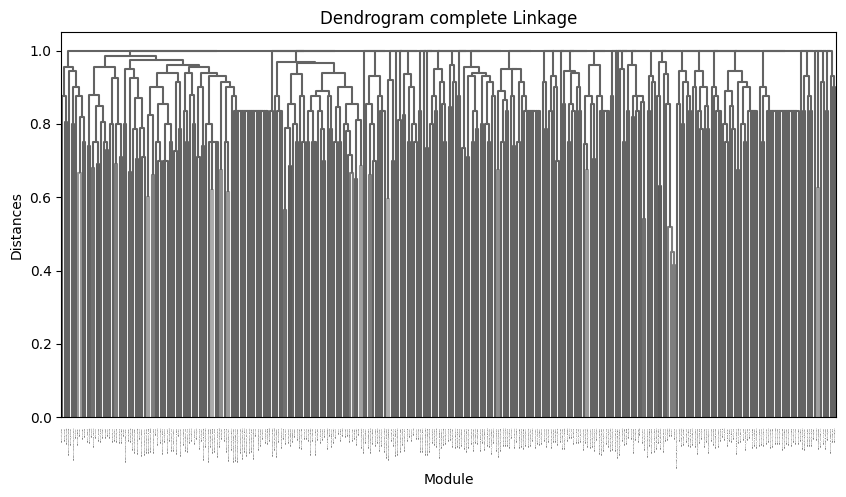
\includegraphics[width=1\textwidth]{img/bab_4/complete_dd.png}
		\caption{Dendogram Complete Linkage }
		\label{fig:dd_complete}
	\end{minipage}\hfill	
\end{figure}

\begin{figure}[htbp]
	\centering
	\begin{minipage}{1\textwidth}
		\centering
		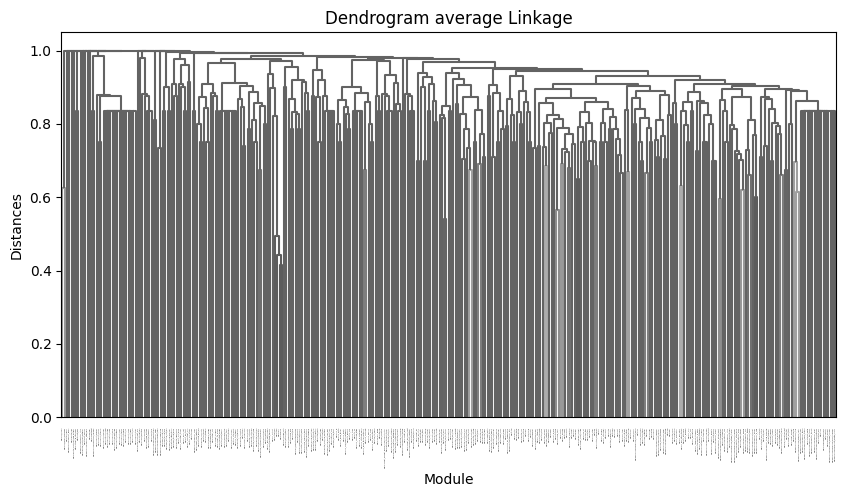
\includegraphics[width=1\textwidth]{img/bab_4/avg_dd.png}
		\caption{Dendogram Average Linkage }
		\label{fig:dd_avg}
	\end{minipage}\hfill	
\end{figure}

\pagebreak


\section{Evaluasi dan Pengujian}
Pada bagian ini, dibahas mengenai evaluasi dan pengujian tentang bagaimana hasil dekomposisi aplikasi monolitik menjadi microservice dengan menggunakan proses Hierarchical Clustering.

\subsection{Pemilihan Partisi}
Banyaknya partisi dan jumlah node, membuat proses pemilihan partisi atau kelompok service terbaik harus dilakukan secara otomatisasi. Untuk mengetahui jumlah partisi yang tepat dilakukan pengukuran dari nilai coupling dan nilai kohesinya yang dihasilkan dari pengelompokan tersebut. Terdapat fungsi yang akan menghitung dari 1 partisi/service hingga jumlah maximum partisi. 

\begingroup
\setlength{\LTleft}{-20cm plus -1fill}
\setlength{\LTright}{\LTleft}
\begin{small}
	\begin{longtable}{|p{4cm}|p{3cm}|p{6cm}|}
		\caption{Daftar Metode untuk pemilihan Partisi}\\
		\hline
		\textbf{Metode / Fungsi} & \textbf{Parameter} & \textbf{Keterangan}\\
		\endfirsthead
		
		\hline  

		mergeClass
		& ct
		 &  Mencari keterhubungan antar partisi dan di dalam partisi berdasarkan tree yang diberikan dari cluster \\

		 \hline  

		 cutTreeToCluster
		& ct
		 & Membuat cluster dari tree yang dihasilkan clustering  \\

		 \hline  

		 NbCalls
		& m, c1, c2
		 & Menghitung jumlah call antar module (Rumus 2.5) \\

		 \hline  
		 CoupP
		 
		& m, c1,c2
		 & Implementasi dari rumus 2.5   \\

		 \hline  

		 InterCoup
		& m
		 & Implementasi dari rumus 2.4 \\

		 \hline
		
		 InterCoh
		& rm
		 & Implementasi dari rumus 2.6  \\

		 \hline
		 
		 FOne
		& m , rm
		 & Implementasi dari rumus 2.3 dan perhitungan skor clustering melalui jumlah partisi, nilai coupling dan nilai cohesion \\

		 \hline
		 calculateFOne
		& z, {\_}n{\_}clusters
		 & Menghitung hasil FOne dengan diberikan z dan jumlah cluster/partisi \\

		 \hline
		 analystCluster
		& z
		 & Melakukan perhitungan calculateFOne dari 1 hingga jumlah maximum cluster/partisi \\ 


		 \hline
		 visualizeQualityCluster
		& qualityCluster, linkageType
		 & Menampilkan plot perbandingan coupling dan cohesion dengan jumlah service  \\

		 \hline
	\end{longtable}
\end{small}
\endgroup

Hasil pemilihan membantu dalam membuat microservice yang memiliki nilai cohesion yang tinggi dan nilai coupling yang rendah. Untuk itu dilakukan perbadingan bagaiman nilai coupling dan cohesion dari jumlah service/partisi yang dimulai dari 1 (monolit) hingga 335 (semua partisi menjadi service individu) dengan setiap linkage yang berbeda.  


\begin{center}
	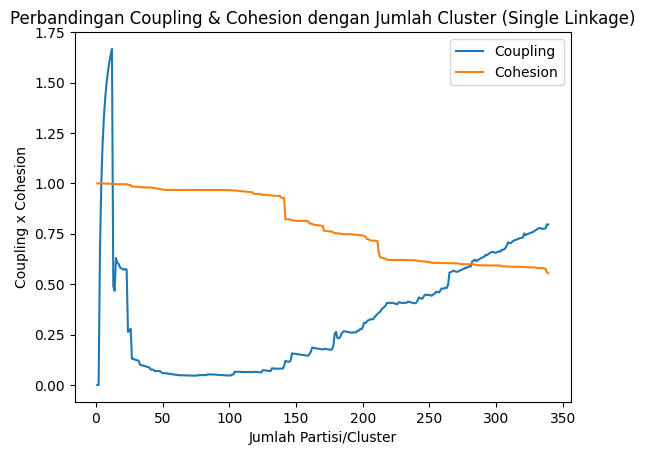
\includegraphics[width=10cm]{img/bab_4/cc_single.png}
	\captionof{figure}{Perbandingan Coupling \& Cohesion menurut pendekatan Single Linkage}
	\label{fig:cc_single}
\end{center}

 Pada grafik \ref{fig:cc_single}, hasil dekomposisi menggunakan linkage single memiliki hasil yang buruk untuk coupling tetapi masih memiliki cohesion yang bagus. Nilai coupling menurun drastis ketika jumlah service mencapai 25 service. Jumlah service yang memiliki nilai coupling rendah dan cohesion yang tinggi berkisar dari 25 service ke atas dan dibawah 150 sevice. Ketika jumlah service melebihi 150 service nilai coupling terus meningkat ketika dan nilai cohesion terus memburuk.
 
 \begin{center}
	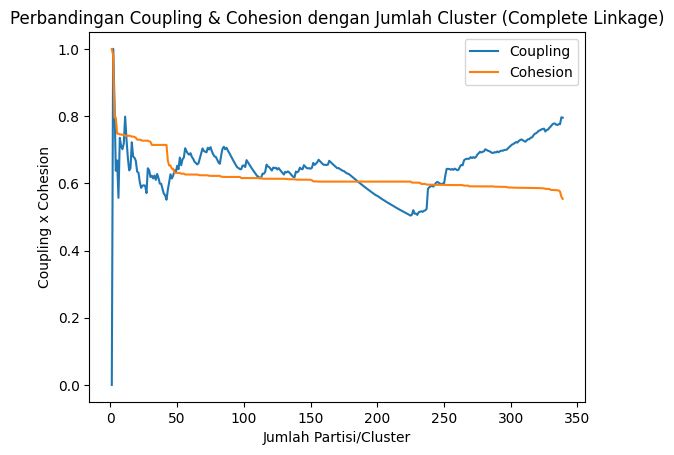
\includegraphics[width=10cm]{img/bab_4/cc_comp.png}
	\captionof{figure}{Perbandingan Coupling \& Cohesion menurut pendekatan Complete Linkage}
	\label{fig:cc_complete}
\end{center}

Pada grafik \ref{fig:cc_complete}, hasil dekomposisi menggunakan linkage complete memiliki coupling yang tinggi sejak dari jumlah service 1 ke atas hingga sekitar 175 service. Nilai Coupling membaik ketika jumlah service mencapai   $\pm 200$  hingga  $\pm 240$, ketika jumlah service melebihi  $\pm 240$ nilai menjadi semakin memburuk coupling. Untuk nilai cohesion turun secara perlahan ketika jumlah service mencapai  $\pm 50$.

\begin{center}
	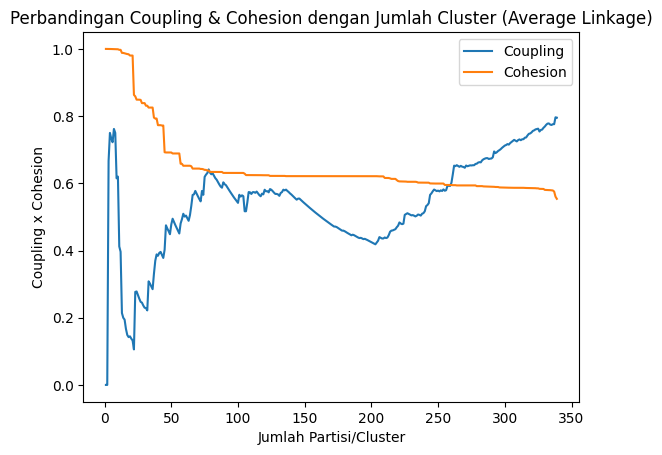
\includegraphics[width=10cm]{img/bab_4/cc_avg.png}
	\captionof{figure}{Perbandingan Coupling \& Cohesion menurut pendekatan Average Linkage }
	\label{fig:cc_avg}
\end{center}

Pada grafik \ref{fig:cc_avg}, hasil dekomposisi menggunakan Average linkage memiliki nilai coupling yang cukup tinggi ketika jumlah service sebesar  $\pm 25$. Nilai coupling meningkat secara tajam ketika jumlah service diatas  $\pm 2$ dan mulai menurun saat jumlah service berkisar  $\pm 100$ - $\pm 210$. Ketika jumlah service melebihi  $\pm 210$ nilai coupling semakin memburuk. Untuk nilai cohesion, memiliki nilai yang tinggi saat jumlah service berkisar  $\pm 2$ -  $\pm 25$, ketika jumlah service diatas  $\pm 25$ nilai cohesion menurun drastis hingga jumlah service  $\pm 75$. Nilai cohesion tidak lagi meningkat dan turun perlahan ketika jumlah service bertambah banyak.

Nilai copling dan cohesion yang dihasilkan bisa dilakukan analisis lebih lanjut seperti melihat nilai maksimum, nilai minimum, dan nilai rata-rata pada nilai coupling dan cohesion untuk setiap linkage.

\begin{table}[ht]
\centering
\begin{tabular}{|c|c|c|c|c|c|c|}
\hline
\multirow{2}{*}{\textbf{Linkage}} & \multicolumn{3}{c|}{\textbf{Coupling}} & \multicolumn{3}{c|}{\textbf{Cohesion}} \\
\cline{2-7}
&  \textbf{MIN} & \textbf{AVG} &  \textbf{MAX} &  \textbf{MIN} &  \textbf{AVG} & \textbf{MAX} \\
\hline
Single & 0.04 & 0.33 & 1.6    & 0.61 & 0.83 & 1 \\
Complete & 0.40 & 0.65 & 1.33 & 0.61 & 0.67 & 0.99 \\
Average & 0.14 & 0.51 & 0.83  & 0.61 & 0.7  & 1 \\
\hline
\end{tabular}
\caption{Tabel  Nilai maximum, rata-rata, dan minimum untuk setiap linkage}
\label{tab:link_stat}
\end{table}

Dari tabel \ref{tab:link_stat} dilihat linkage complete memiliki coupling yang tinggi dan cohesion yang rendah dibandingkan linkage lainnya. Untuk linkage average memiliki nilai coupling dan nilai cohesion yang lebih baik  bila dibandingkan dengan linkage complete tetapi lebih buruk bila dibandingkan dengan linkage single. Nilai  minimum dan maksimum dari cohesion memiliki nilai yang sama tetapi memiliki rata-rata yang berbeda. 

Untuk mengetahui lebih detail bagaimana struktur service dikelompokan, maka untuk setiap linkage, jumlah module dari setiap partisi/service dicari nilai rentang, minimum, dan maksimum untuk setiap jumlah ukuran partisi tertentu (1, 2, 5, 10, 15, 25, 50 , 75, 90, 110, 130, 150, 175, 195, 208 , 220, 232,  245, 275, 290, 305, 325, 335).

\colorlet{mycolor}{blue!20}
\begingroup
\setlength{\LTleft}{-20cm plus -1fill}
\setlength{\LTright}{\LTleft}
\begin{small}
\begin{longtable}{|c|p{4cm}|c|c|c|c|c|}
	\caption{Perbandingan Ukuran Service yang dihasilkan oleh Single Linkage}
	\label{tab:service_stat_single} \\
	\hline
	\textbf{Jumlah} & \textbf{Jumlah Module (Frekuensi)} & \textbf{Coupling} & \textbf{Cohesion} & \multicolumn{3}{c|}{\textbf{Statistik Jumlah Module}} \\
	\cline{5-7}
	&  &  &  & \textbf{MIN} & \textbf{MAX} & \textbf{RANGE} \\
	\hline
	\endfirsthead
	\hline  
	1 & 335(1x) & 0.0 & 1.0 & 335 & 335 & 0 \\   \hline
	\rowcolor{mycolor}
2 & 333(1x), 2(1x) & 0.67 & 1.0 & 2 & 333 & 331 \\   \hline
5 & 326(1x), 5(1x), 2(1x), 1(2x) & 1.33 & 1.0 & 1 & 326 & 325 \\   \hline
10 & 319(1x), 5(1x), 2(3x), 1(5x) & 0.52 & 1.0 & 1 & 319 & 318 \\   \hline
15 & 315(1x), 3(1x), 2(4x), 1(9x) & 0.59 & 1.0 & 1 & 315 & 314 \\   \hline
25 & 299(1x), 5(1x), 3(1x), 2(6x), 1(16x) & 0.19 & 0.98 & 1 & 299 & 298 \\   \hline
50 & 246(1x), 15(1x), 6(2x), 4(1x), 3(1x), 2(11x), 1(33x) & 0.09 & 0.97 & 1 & 246 & 245 \\   \hline
75 & 246(1x), 7(1x), 3(1x), 2(7x), 1(65x) & 0.12 & 0.97 & 1 & 246 & 245 \\   \hline
90 & 241(1x), 2(5x), 1(84x) & 0.2 & 0.97 & 1 & 241 & 240 \\   \hline
110 & 216(1x), 3(2x), 2(6x), 1(101x) & 0.05 & 0.95 & 1 & 216 & 215 \\   \hline
130 & 190(1x), 7(1x), 3(2x), 2(6x), 1(120x) & 0.08 & 0.94 & 1 & 190 & 189 \\   \hline
150 & 169(1x), 3(3x), 2(11x), 1(135x) & 0.1 & 0.91 & 1 & 169 & 168 \\   \hline
175 & 133(1x), 6(1x), 3(3x), 2(17x), 1(153x) & 0.18 & 0.85 & 1 & 133 & 132 \\   \hline
195 & 96(1x), 8(1x), 6(1x), 5(1x), 3(5x), 2(19x), 1(167x) & 0.22 & 0.81 & 1 & 96 & 95 \\   \hline
208 & 66(1x), 11(1x), 8(1x), 6(1x), 5(1x), 4(1x), 3(5x), 2(23x), 1(174x) & 0.28 & 0.76 & 1 & 66 & 65 \\   \hline
220 & 60(1x), 8(1x), 6(1x), 5(2x), 4(1x), 3(5x), 2(23x), 1(186x) & 0.31 & 0.74 & 1 & 60 & 59 \\   \hline
232 & 60(1x), 8(1x), 6(1x), 5(2x), 3(4x), 2(16x), 1(207x) & 0.33 & 0.74 & 1 & 60 & 59 \\   \hline
245 & 54(1x), 8(1x), 5(2x), 3(2x), 2(18x), 1(221x) & 0.36 & 0.72 & 1 & 54 & 53 \\   \hline
275 & 15(1x), 5(2x), 4(2x), 3(6x), 2(20x), 1(244x) & 0.65 & 0.66 & 1 & 15 & 14 \\   \hline
290 & 7(1x), 5(1x), 4(1x), 3(7x), 2(18x), 1(262x) & 0.72 & 0.64 & 1 & 7 & 6 \\   \hline
305 & 6(1x), 4(1x), 3(5x), 2(12x), 1(286x) & 0.75 & 0.64 & 1 & 6 & 5 \\   \hline
325 & 3(1x), 2(8x), 1(316x) & 0.8 & 0.63 & 1 & 3 & 2 \\   \hline
	
\end{longtable}
\end{small}
\endgroup

Pada tabel \ref{tab:service_stat_single} dapat dilihat bahwa jumlah service yang dibuat oleh single linkage tidak merata dalam membagi modulenya, banyak service yang hanya memiliki jumlah modul kecil sekitar 1-3 module tetapi ada satu service yang sangat besar yang memiliki 100-200 module. Service yang memiliki module sangat banyak itu hilang ketika jumlah service / partisi mencapai $\pm 275$, namun nilai coupling dan cohesion ketika jumlah service sebesar $\pm 275$ tidak bagus karena lebih tinggi nilai coupling dibandingkan nilai cohesionnya.


\begingroup
\setlength{\LTleft}{-20cm plus -1fill}
\setlength{\LTright}{\LTleft}
\begin{small}
\begin{longtable}{|c|p{4cm}|c|c|c|c|c|}
		\caption{Perbandingan Ukuran Service yang dihasilkan oleh Complete Linkage}
		\label{tab:service_stat_complete} \\
		\hline
		\textbf{Jumlah} & \textbf{Jumlah Module} & \textbf{Coupling} & \textbf{Cohesion} & \multicolumn{3}{c|}{\textbf{Statistik Jumlah Module}} \\
		\cline{5-7}
		&  &  &  & \textbf{MIN} & \textbf{MAX} & \textbf{RANGE} \\
		\hline
		\endfirsthead
		\hline  
		1 & 335(1x) & 1.0 & 1.0 & 335 & 335 & 0 \\   \hline
2 & 324(1x), 11(1x) & 1.33 & 1.0 & 11 & 324 & 313 \\   \hline
5 & 212(1x), 88(1x), 17(1x), 11(1x), 7(1x) & 0.68 & 0.96 & 7 & 212 & 205 \\   \hline
10 & 132(1x), 88(1x), 31(1x), 17(2x), 16(1x), 11(1x), 8(2x), 7(1x) & 0.41 & 0.93 & 7 & 132 & 125 \\   \hline
15 & 107(1x), 88(1x), 31(1x), 17(2x), 16(1x), 11(1x), 10(1x), 8(2x), 7(2x), 4(1x), 2(2x) & 0.6 & 0.82 & 2 & 107 & 105 \\   \hline
25 & 88(1x), 46(1x), 31(1x), 17(2x), 16(2x), 11(1x), 10(2x), 8(4x), 7(2x), 5(1x), 4(3x), 2(5x) & 0.62 & 0.75 & 2 & 88 & 86 \\   \hline
50 & 67(1x), 25(1x), 17(2x), 16(1x), 15(1x), 10(2x), 8(6x), 7(1x), 6(4x), 5(3x), 4(4x), 3(6x), 2(12x), 1(6x) & 0.65 & 0.74 & 1 & 67 & 66 \\   \hline
75 & 34(1x), 21(1x), 16(1x), 13(1x), 9(1x), 8(4x), 7(2x), 6(7x), 5(4x), 4(14x), 3(8x), 2(23x), 1(8x) & 0.67 & 0.7 & 1 & 34 & 33 \\   \hline
90 & 19(1x), 16(1x), 9(2x), 8(5x), 7(3x), 6(5x), 5(4x), 4(15x), 3(12x), 2(33x), 1(9x) & 0.64 & 0.68 & 1 & 19 & 18 \\   \hline
110 & 19(1x), 16(1x), 9(1x), 8(2x), 7(3x), 6(3x), 5(6x), 4(11x), 3(17x), 2(46x), 1(19x) & 0.67 & 0.67 & 1 & 19 & 18 \\   \hline
130 & 16(2x), 7(1x), 6(4x), 5(6x), 4(11x), 3(22x), 2(48x), 1(36x) & 0.61 & 0.66 & 1 & 16 & 15 \\   \hline
150 & 16(1x), 15(1x), 6(3x), 5(3x), 4(5x), 3(26x), 2(62x), 1(49x) & 0.68 & 0.65 & 1 & 16 & 15 \\   \hline
175 & 16(1x), 15(1x), 5(1x), 4(5x), 3(20x), 2(72x), 1(75x) & 0.65 & 0.65 & 1 & 16 & 15 \\   \hline
195 & 14(1x), 8(1x), 5(1x), 4(4x), 3(19x), 2(66x), 1(103x) & 0.61 & 0.65 & 1 & 14 & 13 \\   \hline
208 & 9(1x), 5(1x), 4(4x), 3(19x), 2(65x), 1(118x) & 0.57 & 0.65 & 1 & 9 & 8 \\   \hline
220 & 5(1x), 4(3x), 3(20x), 2(62x), 1(134x) & 0.54 & 0.65 & 1 & 5 & 4 \\   \hline
232 & 5(1x), 4(3x), 3(17x), 2(56x), 1(155x) & 0.55 & 0.65 & 1 & 5 & 4 \\   \hline
245 & 4(1x), 3(11x), 2(65x), 1(168x) & 0.64 & 0.64 & 1 & 4 & 3 \\   \hline
275 & 3(4x), 2(52x), 1(219x) & 0.69 & 0.64 & 1 & 3 & 2 \\   \hline
290 & 3(2x), 2(41x), 1(247x) & 0.71 & 0.64 & 1 & 3 & 2 \\   \hline
305 & 3(1x), 2(28x), 1(276x) & 0.78 & 0.63 & 1 & 3 & 2 \\   \hline
325 & 2(10x), 1(315x) & 0.81 & 0.62 & 1 & 2 & 1 \\   \hline
	\end{longtable}
\end{small}
\endgroup

Pada tabel \ref{tab:service_stat_complete} dapat dilihat bahwa jumlah service yang dibuat oleh complete linkage cenderung membentuk service yang besar karena dilihat dari jumlah module yang dimiliki oleh setiap service, namun nilai rentang dari besarnya sebuah service lebih kecil. Di sisi lain nilai coupling dan cohesion yang dihasilkan buruk walaupun jumlah service masih sedikit bila dibandingkan dengan linkage lain.

\begingroup
\setlength{\LTleft}{-20cm plus -1fill}
\setlength{\LTright}{\LTleft}
\begin{small}
\begin{longtable}{|c|p{4cm}|c|c|c|c|c|}
	\caption{Perbandingan Ukuran Service yang dihasilkan oleh Average Linkage}
	\label{tab:service_stat_average} \\
	\hline
	\textbf{Jumlah} & \textbf{Jumlah Module} & \textbf{Coupling} & \textbf{Cohesion} & \multicolumn{3}{c|}{\textbf{Statistik Jumlah Module}} \\
	\cline{5-7}
	&  &  &  & \textbf{MIN} & \textbf{MAX} & \textbf{RANGE} \\
	\hline
	\endfirsthead
	\hline 
	1 & 335(1x) & 0.0 & 1.0 & 335 & 335 & 0 \\   \hline
2 & 333(1x), 2(1x) & 0.67 & 1.0 & 2 & 333 & 331 \\   \hline
5 & 329(1x), 2(2x), 1(2x) & 0.72 & 1.0 & 1 & 329 & 328 \\   \hline
10 & 305(1x), 20(1x), 2(2x), 1(6x) & 0.45 & 1.0 & 1 & 305 & 304 \\   \hline
15 & 293(1x), 20(1x), 6(1x), 2(4x), 1(8x) & 0.18 & 0.98 & 1 & 293 & 292 \\   \hline
25 & 198(1x), 51(1x), 20(1x), 11(1x), 9(1x), 8(1x), 5(3x), 4(1x), 2(4x), 1(11x) & 0.25 & 0.9 & 1 & 198 & 197 \\   \hline
50 & 74(1x), 54(1x), 17(1x), 16(2x), 15(1x), 14(1x), 11(1x), 8(1x), 7(1x), 6(3x), 5(6x), 4(1x), 3(5x), 2(11x), 1(14x) & 0.33 & 0.81 & 1 & 74 & 73 \\   \hline
75 & 29(1x), 28(1x), 17(2x), 16(1x), 12(2x), 11(1x), 10(2x), 8(1x), 7(2x), 6(4x), 5(5x), 4(5x), 3(7x), 2(20x), 1(21x) & 0.42 & 0.72 & 1 & 29 & 28 \\   \hline
90 & 29(1x), 19(1x), 16(1x), 13(1x), 11(2x), 10(1x), 7(2x), 6(9x), 5(3x), 4(11x), 3(7x), 2(27x), 1(24x) & 0.45 & 0.72 & 1 & 29 & 28 \\   \hline
110 & 29(1x), 19(1x), 15(1x), 11(2x), 8(1x), 7(2x), 6(8x), 5(4x), 4(7x), 3(8x), 2(33x), 1(42x) & 0.41 & 0.7 & 1 & 29 & 28 \\   \hline
130 & 16(1x), 15(1x), 13(1x), 11(1x), 10(1x), 8(1x), 6(7x), 5(5x), 4(2x), 3(14x), 2(49x), 1(47x) & 0.47 & 0.67 & 1 & 16 & 15 \\   \hline
150 & 13(2x), 10(2x), 8(1x), 6(5x), 5(5x), 4(1x), 3(16x), 2(56x), 1(62x) & 0.56 & 0.67 & 1 & 13 & 12 \\   \hline
175 & 13(2x), 10(1x), 8(1x), 6(4x), 5(5x), 4(1x), 3(14x), 2(49x), 1(98x) & 0.49 & 0.67 & 1 & 13 & 12 \\   \hline
195 & 13(1x), 10(2x), 8(1x), 6(3x), 5(4x), 4(1x), 3(11x), 2(47x), 1(125x) & 0.46 & 0.67 & 1 & 13 & 12 \\   \hline
208 & 13(1x), 10(1x), 8(1x), 6(2x), 5(4x), 4(2x), 3(10x), 2(47x), 1(140x) & 0.44 & 0.67 & 1 & 13 & 12 \\   \hline
220 & 10(1x), 6(1x), 5(5x), 4(3x), 3(11x), 2(50x), 1(149x) & 0.49 & 0.66 & 1 & 10 & 9 \\   \hline
232 & 6(1x), 5(4x), 4(2x), 3(14x), 2(48x), 1(163x) & 0.52 & 0.65 & 1 & 6 & 5 \\   \hline
245 & 5(1x), 4(4x), 3(11x), 2(52x), 1(177x) & 0.56 & 0.65 & 1 & 5 & 4 \\   \hline
275 & 3(8x), 2(44x), 1(223x) & 0.68 & 0.64 & 1 & 3 & 2 \\   \hline
290 & 3(6x), 2(33x), 1(251x) & 0.71 & 0.64 & 1 & 3 & 2 \\   \hline
305 & 3(4x), 2(22x), 1(279x) & 0.76 & 0.63 & 1 & 3 & 2 \\   \hline
325 & 2(10x), 1(315x) & 0.81 & 0.62 & 1 & 2 & 1 \\   \hline
\end{longtable}
\end{small}
\endgroup

Pada tabel \ref{tab:service_stat_average} dapat dilihat bahwa jumlah service dibuat oleh average linkage memiliki service yang tidak terlalu besar bila dilihat dari nilai maksimum jumlah module dan terdapat service yang berukuran kecil (1 modul). Dari nilai coupling dan nilai cohesion, average linkage memiliki nilai yang bagus karena nilai coupling masih dibawah nilai cohesion. 

Dari hasil perbandingan ukuran service yang dihasilkan oleh masing-masing linkage pada kasus dekomposisi aplikasi monolitik Odoo, menunjukan bahwa complete linkage tidak cocok untuk melakukan dekomposisi karena service yang dibentuk besar dan memiliki nilai coupling tinggi. Sedangkan single linkage kurang ideal walaupun memiliki coupling yang rendah dan cohesion yang tinggi namun service yang dibuat tidak dikelompokan secara seimbang dan memiliki nilai rentang yang besar, karena ada service yang memiliki jumlah sangat besar. Untuk Average linkage dapat membentuk service yang ideal karena ukuran service tidak terlalu besar dilihat dari nilai rentangnya dan memiliki nilai couplingnya rendah serta nilai cohesionnya cukup tinggi. 

Pemilihan jumlah service yang ideal pada Average linkage, tidak bisa ditentukan secara pasti karena terdapat \textit{trade-off} untuk setiap kenaikan jumlah service. Oleh karena itu rentang jumlah service yang ideal adalah bisa dari 175, 195, 208, 220, 232 , 245. Jumlah service yang tidak ideal adalah dibawah $\pm 150 / \pm 175$ service karena nilai rentang service cukup tinggi yaitu diatas 12 module dan diatas $\pm 245$ service karena nilai coupling lebih tinggi dibandingkan nilai cohesionnya. \\


\subsection{Dekomposisi Monolitik \textit{ ke Microservice}}
Pada bagian ini menjelaskan bagaimana penerapan microservice dengan menggunakan hasil dekomposisi yang dihasilkan oleh hierarchical clustering. 

\subsubsection{Pemilihan Service}
Pada tugas akhir ini memilih untuk menggunakan hasil Hierarchical Clustering dengan Average Linkage dengan jumlah service sebesar  $\pm 220$. Hasil evaluasi sebelumnya menunjukan nilai coupling sebesar 0.66, nilai cohesion sebesar 0.49 dan nilai rentang sebesar 9. Detail isi dari setiap module untuk setiap partisi yang dikelompokan dapat dilihat pada Tabel. \ref{tab:daftar_module_final} 

\begingroup
\setlength{\LTleft}{-20cm plus -1fill}
\setlength{\LTright}{\LTleft}
\begin{small}
	\begin{longtable}{|c|p{14cm}|}
		\caption{Daftar Module untuk Setiap Partisi}
		\label{tab:daftar_module_final}\\
		\hline
		\textbf{Partisi} & \textbf{Daftar Module}
		\\
		\endfirsthead
		\hline  
		1 & auth{\_}totp{\_}mail \\ \hline
		2 & base.models.res{\_}users, fleet, sales{\_}team, membership \\ \hline
		3 & auth{\_}signup, portal \\ \hline
		4 & web \\ \hline
		5 & hr{\_}work{\_}entry{\_}contract, resource, hr{\_}work{\_}entry, hr{\_}holidays, hr{\_}contract \\ \hline
		6 & base.models.ir{\_}http \\ \hline
		7 & base.models.res{\_}config, digest, base{\_}geolocalize, auth{\_}ldap, auth{\_}password{\_}policy \\ \hline
		8 & base.models.res{\_}partner, uom, base{\_}sparse{\_}field \\ \hline
		9 & website{\_}sale{\_}loyalty, sale{\_}loyalty \\ \hline
		10 & loyalty, sale, account, product, analytic, hr{\_}expense, purchase{\_}stock, purchase, project, lunch \\ \hline
		13 & delivery, delivery{\_}mondialrelay \\ \hline
		14 & stock, point{\_}of{\_}sale, mrp \\ \hline
		20 & website{\_}event{\_}track, website{\_}event, website{\_}event{\_}exhibitor, website{\_}event{\_}meet, website{\_}event{\_}track{\_}quiz \\ \hline
		22 & event, link{\_}tracker, mass{\_}mailing \\ \hline
		25 & website{\_}forum, website{\_}slides, website{\_}blog, website{\_}crm{\_}partner{\_}assign \\ \hline
		32 & base.models.image{\_}mixin, base.models.avatar{\_}mixin \\ \hline
		35 & hr{\_}recruitment, hr \\ \hline
		46 & google{\_}calendar, microsoft{\_}calendar \\ \hline
		56 & portal{\_}rating \\ \hline
		57 & base{\_}install{\_}request, base.models.ir{\_}module, base.wizard.base{\_}module{\_}uninstall, base{\_}import{\_}module, base.wizard.base{\_}export{\_}language \\ \hline
		58 & base.models.ir{\_}qweb \\ \hline
		59 & base.models.ir{\_}ui{\_}view, base.models.report{\_}layout \\ \hline
		80 & pos{\_}discount, pos{\_}sale \\ \hline
		101 & base.models.res{\_}bank \\ \hline
		133 & transifex \\ \hline
		159 & microsoft{\_}outlook, google{\_}gmail \\ \hline
		181 & sale{\_}mrp \\ \hline
		216 & pos{\_}loyalty \\ \hline
		217 & mass{\_}mailing{\_}event{\_}sms \\ \hline
		218 & spreadsheet{\_}dashboard \\ \hline
		219 & crm{\_}livechat \\ \hline
		220 & sale{\_}purchase{\_}stock \\ \hline
	\end{longtable}
\end{small}
\endgroup

Service yang dipilih untuk dilakukan implementasi dekomposisi yaitu  service / partisi ke-10  pada module addons.product dan partisi ke-14 pada modul  addons.point{\_}of{\_}sale. Di dalam module ini terdapat beberapa model yang dapat dilakukan dekomposisi berikut isi model dari module yang dipilih ditampilkan pada Tabel. \ref{fig:findme}.



% Tabel model dan nilai weight dll 

\subsubsection{\textit{Endpoint API}}
Pada Tabel \ref{tab:endpoint-api} dijelaskan endpoint dan routing yang dipakai dalam masing-masing service. Endpoint tersebut digunakan untuk melakukan uji beban dan pengukuran penggunaan sumber daya dengan sistem monolitik yang sudah dibuat.  

Untuk Client berkomunikasi dengan service maka harus melalui API Gateway dan setiap service untuk mencari service lainnya dapat diarahkan oleh API Gateway. API Gateway membuat rute berdasarkan URL path yang sudah dikonfigurasi sebelumnya serta service dan API Gateway berada di jaringan yang sama.

Berikut IP Address dan port yang digunakan setiap service:
\begin{enumerate}[leftmargin=1.3cm]
	\item Kong Gateway $\rightarrow$ 172.18.0.5:8000
	\item Monolitik $\rightarrow$ 172.18.0.55:8069
	\item Product Service $\rightarrow$ 172.18.0.51:1323
	\item Point of Sale Service $\rightarrow$ 172.18.0.52:1323
\end{enumerate}

\begingroup
\setlength{\tabcolsep}{6pt} % Adjust the column separation as needed
\begin{small}
	\begin{longtable}{|c|p{3cm}|p{3cm}|p{6cm}|}
	\caption{Tabel Endpoint API} \label{tab:endpoint-api} \\
	\hline
	\textbf{Metode} & \textbf{Route} & \textbf{Body} & \textbf{Keterangan} \\
	\hline
	\endfirsthead
	
	\multicolumn{4}{c}%
	{{\tablename\ \thetable{} -- Lanjutan dari halaman sebelumnya}} \\
	\hline
	\textbf{Metode} & \textbf{Route} & \textbf{Body} & \textbf{Keterangan} \\
	\hline
	\endhead
	
	\hline \multicolumn{4}{|r|}{{Lanjutan di halaman berikutnya}} \\ \hline
	\endfoot
	
	\hline
	\endlastfoot
	
	\multicolumn{4}{|c|}{Monolith (/web/session/*)} \\
	\hline
	POST & /authenticate & JSON, Format: JSON-RPC & Melakukan sesi autentikasi pengguna \\
	\hline
	POST & /destroy & JSON, Format: JSON-RPC & Menghilangkan sesi autentikasi pengguna \\
	\hline
	
	\multicolumn{4}{|c|}{Point of Sales Service (/web/dataset/call\_kw/pos.category/*)} \\
	\hline
	POST & /read & JSON, Format: JSON-RPC & Mendapatkan data Point Of Sale Category \\
	\hline
	POST & /create & JSON, Format: JSON-RPC & Menambahkan data Point Of Sale Category \\
	\hline
	
	\multicolumn{4}{|c|}{Product Service (/web/dataset/call\_kw/product.tag/*)} \\
	\hline
	POST & /read & JSON, Format: JSON-RPC & Mendapatkan data Tag pada product\\
	\hline
	POST & /create & JSON, Format: JSON-RPC & Menambahkan  data Tag pada product \\
	\hline
	
	\end{longtable}
	\end{small}
\endgroup

\subsubsection{ Daftar Class}
Pada bagian ini dijelaskan class yang digunakan PosCategory dan ProductTag :

\begin{longtable}{|c|p{3cm}|p{3cm}|p{4cm}|}
	\caption{Tabel class yang digunakan}
	\label{tab:daftar-class}\\
	\hline
	\textbf{Class} & \textbf{Atribut} & \textbf{Tipe Data} & \textbf{Keterangan} \\
	\hline
	\endfirsthead
	\hline
	\multicolumn{4}{|c|}{\textbf{Dilanjutkan di Halaman Selanjutnya}} \\
	\hline
	\textbf{Class} & \textbf{Atribut} & \textbf{Tipe Data} & \textbf{Keterangan} \\
	\hline
	\endhead
	\hline
	\multicolumn{4}{|c|}{\textbf{Lanjutan Isi Tabel Sebelumnya}} \\
	\hline
	\endfoot
	\hline
	\endlastfoot
	ResUser & UID & int & Class yang menyimpan informasi mengenai pengguna aplikasi/ Odoo. Hampir semua aktivitas pengguna harus dicatat dan harus divalidasi melalui GroupID. Informasi ini dimasukan dari nilai JWT yang disimpan client \\
	\cline{2-3}
	& DisplayName & string & \\
	\cline{2-3}
	& GroupID & int & \\
	\hline
	AccessControlList & GroupID & int & Class yang menyimpan hak akses suatu model atau resource dan dapat dilihat nilai GroupID. Hak akses ini dikomunikasikan dalam waktu tertentu oleh masing-masing service.  \\
	\cline{2-3}
	& ModelID & int & \\
	\cline{2-3}
	& Read & bool & \\
	\cline{2-3}
	& Write & bool & \\
	\cline{2-3}
	& Create & bool & \\
	\cline{2-3}
	& Unlink & bool & \\
	\hline

	\multicolumn{4}{|c|}{\textbf{Point of Sales}} \\
	\hline
	PosCategory & ID & uint & PosCategory atau Point of Sales Category adalah untuk membantu mengelola barang yang yang didagangkan melalui Point of Sale. Kategori ini bisa memiliki tingkatan kategori dan gambar dari kategori tersebut. \\
	\cline{2-3}
	& ParentID & uint & \\
	\cline{2-3}
	& Name & string & \\
	\cline{2-3}
	& Sequence & int & \\
	\cline{2-3}
	& Image &  PosCategoryImage & \\
	\cline{2-3}
	& CreateAt & Timestamp & \\
	\cline{2-3}
	& CreatUID & ResUser & \\
	\cline{2-3}
	& WriteAt & Timestamp & \\
	\cline{2-3}
	& WriteUID & ResUser & \\

	\hline
	PosCategoryImage & UID & int & Merupakan object yang menyimpan informasi gambar yang dimiliki oleh kategori. Gambar disimpan didatabase dan memiliki IdAttachment yang diketahui oleh sistem monolith\\
	\cline{2-3}
	& ImageBase64 & string & \\
	\cline{2-3}
	& AttachmentId & int & \\
	\cline{2-3}
	& ImageSizeByte & int & \\
	\hline

	\multicolumn{4}{|c|}{\textbf{Product}} \\
	\hline
	ProductTag & ID & uint & Product Tag adalah model yang mengelola banyak label untuk memudahkan pencarian disuatu  produk. Product Tag memiliki satu nama yang unik tetapi bisa dimiliki oleh banyak produk template atau produk-produk (varian) \\
	\cline{2-3}
	& Color & uint & \\
	\cline{2-3}
	& Name & string & \\
	\cline{2-3}
	& CreateAt & Timestamp & \\
	\cline{2-3}
	& CreatUID & ResUser & \\
	\cline{2-3}
	& WriteAt & Timestamp & \\
	\cline{2-3}
	& WriteUID & ResUser & \\
	\cline{2-3}
	& ProductTemplate & int[] & \\
	\cline{2-3}
	& ProductProduct & int[] & \\
	\hline
\end{longtable}

\subsubsection{\textit{Docker} }
Pada tugas akhir ini menggunakan teknologi Docker untuk membangun dan mendistribusikan aplikasi dalam bentuk container. Setiap service akan terhubung pada jaringan yang sama. Setiap service termasuk aplikasi monolih memiliki image yang bisa dilakukan deployment antar platform. 

Berikut adalah inisialisasi untuk membuat container dari masing-masing service, setiap serive berada di jaringan internal odoo yang sudah ditentukan sebelum. Tujuannya agar pemetaan service bisa dilukan dengan target ip yang konsisten.

\begin{lstlisting}[style=mystyle, language=sh, caption={Shell Script untuk pembuatan jaringan }]
$ docker network create --subnet=172.18.0.0/16 mono-net
$ docker network create --subnet=172.18.0.0/16 odoo-ms-net	
\end{lstlisting} 

\begin{lstlisting}[style=mystyle, language=sh, caption={Shell Script untuk pembuatan container }]
$ docker run -d --name odoo-kong-gateway \
	--network=odoo-ms-net \
	--ip 172.18.0.5 \
	-v "$(pwd):/kong/declarative/" \
	-e "KONG_DATABASE=off" \
	-e "KONG_DECLARATIVE_CONFIG=/kong/declarative/kong.yml" \
	-e "KONG_PROXY_ACCESS_LOG=/dev/stdout" \
	-e "KONG_ADMIN_ACCESS_LOG=/dev/stdout" \
	-e "KONG_PROXY_ERROR_LOG=/dev/stderr" \
	-e "KONG_ADMIN_ERROR_LOG=/dev/stderr" \
	-e "KONG_ADMIN_LISTEN=0.0.0.0:8001" \
	-p 8000:8000 \
	-p 8001:8001 \
	-p 8002:8002 \
	-p 8003:8003 \
	kong/kong-gateway:latest 
$ docker run -v "/ubuntu/local":/home/odoo/shared_data --net odoo-ms-net  --ip 172.18.0.55 --name odoo-mono -p :8069  -d odoo-mono
$ docker run --net odoo-ms-net --ip 172.18.0.54 --name odoo-mariadb -e MYSQL_ROOT_PASSWORD=mariadb -p 3306:3306 -d mariadb 
$ docker run --net odoo-ms-net  --ip 172.18.0.11 --name postgres-odoo -e POSTGRES_PASSWORD=postgres -p 5432:5432 -d postgres
\end{lstlisting} 

\subsubsection{ \textit{Kong}}
Proses selanjutnya yaitu membuat Api Gateway, tugas akhir ini menggunakan Kong sebagai api gateway. Konfigurasi Kong yang digunakan tidak menggunakan database tetapi berupa konfigurasi statik berupa file .yml/.json. Tugas akhir ini menggunakan yml.

Endpoint yang diset adalah keterangan service (ip address,port,protocol) dan routing (metode, apakah host di rewrite ketika dialihkan). Dengan api gateway client hanya perlu mengetahui endpoint pusat kong yaitu :8000. Ketika pencarian rute url tidak ditemukan maka otomatis diarah service monolith (odoo-mono).

\begin{lstlisting}[style=mystyle, language=sh, caption={Konfigurasi Service Monolith }]
- name: odoo-mono
  port: 8069
  protocol: http
  host: 172.18.0.55
  routes:
  - name: odoo-mono-route
    methods:
        - GET
        - POST
        - PUT
        - DELETE
        - PATCH
        - HEAD
        - OPTION
    paths:
    - /
    strip_path: false
    preserve_host: true
\end{lstlisting} 

\begin{lstlisting}[style=mystyle, language=sh, caption={Konfigurasi Service Point of Sale }]
- name: odoo-pos
  port: 1323
  protocol: http
  host: 172.18.0.51
  path: /jsonrpc
  routes:
  - name: odoo-pos-route
    methods:
        - POST
    paths:
    - /web/dataset/call_kw/pos.category/create
    - /web/dataset/call_kw/pos.category/write
    - /web/dataset/call_kw/pos.category/unlink
    - /web/dataset/call_kw/pos.category/read
    strip_path: false
    preserve_host: true
\end{lstlisting} 

\begin{lstlisting}[style=mystyle, language=sh, caption={Konfigurasi Service Product }]
- name: odoo-product
  port: 1323
  protocol: http
  host: 172.18.0.52
  path: /jsonrpc
  routes:
  - name: odoo-product-route
    methods:
        - POST
    paths:
    - /web/dataset/call_kw/product.tag/create
    - /web/dataset/call_kw/product.tag/write
    - /web/dataset/call_kw/product.tag/unlink
    - /web/dataset/call_kw/product.tag/read
    strip_path: false
    preserve_host: true	
\end{lstlisting} 
	
\subsubsection{Penerapan JSON Web  Token(JWT)}
Perubahan migrasi arsitektur dari monolith ke microservice, membuat diperlukan sistem pengelolaan hak akses yang stateless. Sehingga service tidak sering harus berkomunikasi satu sama lain terutama pada hal informasi yang sama. Token disimpan didalam cookie client, sehingga baik dari client yang melalui user-interface atau pun secara langsung API, bisa diidentifikasi selama client tersebut memberikan token di cookie ketika meminta data.

\begin{lstlisting}[style=mystyle, language=java, caption={Isi data berupa JSON di JWT}]
{
  "uid": 2,
  "user_context": {
    "lang": "en_US",
    "tz": "Europe/Brussels",
    "uid": 2
  },
  "db": "odoo_db",
  "company_id": 1,
  "partner_id": 3,
  "group_id": [
    2,22,7,34,48
  ],
  "exp": 1692576855
}
\end{lstlisting} 


Untuk menambahkan JWT bisa dituliskan pada proses login sendiri seperti pada \ref{fig:sessionRoute} file py yaitu addons / web/ controlers / session.py . Pada route  /web/session/authenticate 
\begin{figure}[htbp]
	\centering
	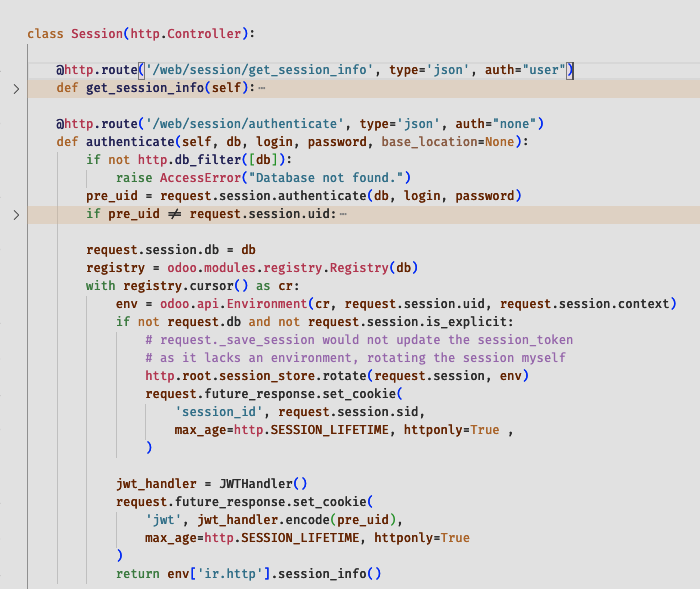
\includegraphics[width=0.7\textwidth]{img/bab_4/sessionRoute.png}
	\caption{Penggalan Kode untuk disisipi proses JWT}
	\label{fig:sessionRoute}
\end{figure}

Data yang disimpan oleh JWT penting diketahui secara umum service, seperti pengguna, konteks pengguna(bahasa, zona waktu), perusahaan, dan database(db).  Perusahaan dan database diperlukan karena odoo memiliki fitur untuk memilih database dan untuk memanggil  aplikasi monolith(Odoo) harus diketahui databasenya. JWT ini dibuat oleh aplikasi monolith ketika login dan dihapus ketika logout atau sesi sudah habis(exp). Masa hidup JWT sama dengan masa hidup session-token yaitu 3 bulan.

Untuk menghancurkan sesi maka ditambahakan mekanisme berupa cookie yang menunjukan bahwa jwt sudah tidak valid. Kemudian cookie tersebut akan dicek oleh fungsi di odoo / http.py / Request.savesession untuk menghapus cookie dengan nama 'jwt' . 
\begin{figure}[htbp]
	\centering
	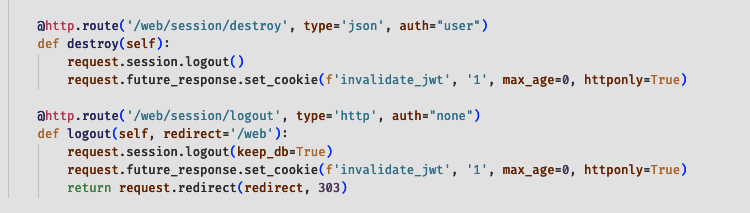
\includegraphics[width=0.8\textwidth]{img/bab_4/triggerCookieDel.png}
	\caption{Potongan Kode untuk memberikan validasi bawah JWT tidak valid}
	\label{fig:example}
\end{figure}

\begin{figure}[htbp]
	\centering
	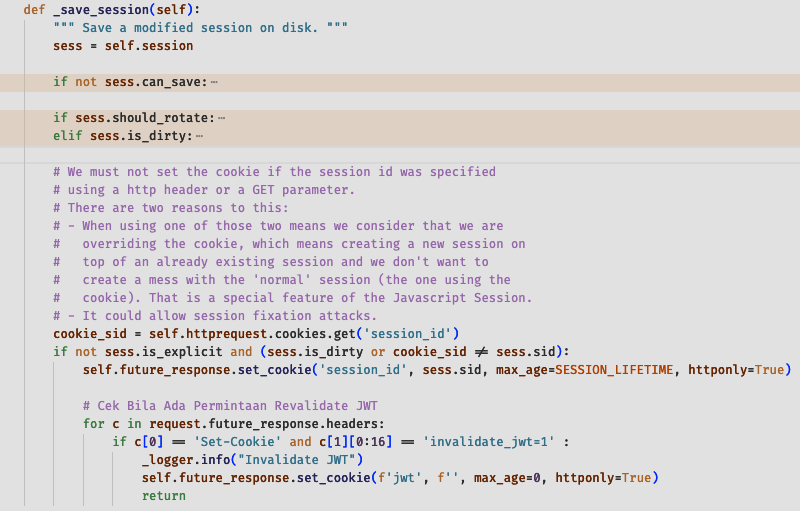
\includegraphics[width=0.8\textwidth]{img/bab_4/removeCookie.png}
	\caption{Potongan Kode untuk memberikan validasi bawah JWT tidak valid}
	\label{fig:example}
\end{figure}

Pada gambar \ref{fig:jwt_proof}, merupakan tangkapan layar pada ResponseHeader melalui DevTools di Browser. Pada gambar bagian kiri terdapat bagian response ketika cookie dengan key JWT berhasil di'set' oleh server, dan pada gambar sisi kanan menunjukan reponse ketika cookie pada JWT dihilangkan.


\subsubsection{Pola Strangle}
Perubahan arsitektur dari aplikasi monolith menjadi microservice membutuhkan banyak resiko dan sumber daya untuk itu perubahan sebaiknya tidak mengurangi atau memperburuk aplikasi yang sudah jadi. Setiap proses bisnis odoo selalu mengimplementasikan class MetaModel. MetaModel membantu pengembang bisa membuat cepat aplikasi tapi MetaModel memiliki keterkaitan dengan model lainnya tinggi. Model di Odoo bisa mengelola data seperti menyimpan di database, memanggil model lainnya, data untuk tampilan(Frontend), dan hal lainnya.

Di MetaModel terdapat fungsi umum dan fungsi internal yang bisa di'override'. Fungsi tersebut dapat dijadikan sebuah adapter. Fungsi utama yang selalu ada pada model yaitu fungsi create, browse, unlink, \_read dan read. Fungsi dan metode tersebut berfungsi untuk mengelola data. Model Adapter dibuat untuk mengabstraksi pengelolaan data sehingga implementasi logic bisa dipindahkan atau dialihkan ke service lainnya dan dikomunikasikan melalui panggilan RPC.  

Adapter yang dibuat juga memiliki kemampuan mengelola datanya karena data yang simpan hanyalah data yang diperlukan oleh sistem lainnya, seperti ID yang digunakan sebagai referensi hubungan antar module. Adapter akan mengelola data secara langsung dari database karena adapter harus berkomunikasi dahulu kepada service yang memiliki tanggung jawab data tersebut.

Ketika ditemukan bahwa data yang berbeda maka dilakukan Update dan didapatkan bila tidak ada, namun ketika data tersebut sebelumnya ada tetapi ketika dicek ditemukan tidak ada. Maka adapter akan mencoba menghapus data tersebut, hal ini akan membuat efek berkelanjutan dengan sistem yang lain. Bila ternyata data tersebut tidak dapat dihapus maka data tersebut hanya bisa didapatkan dan tidak bisa diubah.

Pada pemisahan  model PosCategory, proses penyimpanan data baru dapat memiliki sebuah gambar. Untuk itu ketika ada penyimpana gambar maka gambar disimpan pada database untuk dicatat dan kemudian dikirimkan kepada aplikasi monolith untuk data melalui model ir.attachment di RPC agar gambar bisa diakses melalui web. Setiap model pada Odoo memiliki hak akses kepada grup tertentu. Hak akses bisa diasumsikan jarang berubah untuk karena itu agar service mengetahui apakah seorang user memiliki hak akses. Service memiliki jadwal melaui cron job untuk mengecheck apakah ada akses grup baru.

Service diminta untuk mencatat siapa dan kapan data berubah. Sehingga ada relasi kepada res.user relasi ini hanya memiliki ID, DisplayName, dan GroupID. Informasi ini didapatkan melalui data JWT yang dikirimkan oleh client sebelumnya.

\subsubsection{Analisis Hasil Dekomposisi}
Jelaskan module  Pos  Pos Categ, ini contoh kalo hanya satu

Jelaskan module  Product Product.tag, contoh yang ada hubungannya

Jelaskan hasil implementasi dengan UI web bahw amodule , bahwa bisa dilakukan pola strange, ss Postman dan 
